\documentclass[
%draft, 
12pt, a4paper, oneside]{ctexart}
\tolerance=20000
\usepackage{metalogo}
\usepackage{tikz}
\usepackage{float}
\usepackage{forest}
\usepackage{dirtree}
\usepackage{listings}
\usepackage{amsmath, amsthm, amssymb, appendix, bm, mathrsfs, graphicx, upgreek, parskip}
\usepackage[dvipsnames]{xcolor}
\usepackage{unicode-math}
\usepackage{subcaption}
\graphicspath{{image/}}
\usepackage[square, super,sort&compress]{natbib} % 引用宏包
%\setmathfont{TeX Gyre Termes Math}
%\usepackage{isomath} % 导入isomath包
%\usepackage{newtx} % 提供\uppartial
\usepackage{etoolbox}

% 带圈数字
\usepackage{fontspec}
% \setmathfont{XITS Math}
% 定义带圈数字字体(不更改全局字体)
\newfontfamily{\circlefont}{Segoe UI Symbol}
\setmonofont{Consolas}[Scale = 0.9]

% listings设置
\definecolor{lightgray}{rgb}{0.95,0.95,0.95}
\lstset{
  backgroundcolor = \color{lightgray},      % 浅灰色背景
  basicstyle = \fontsize{10}{11}\ttfamily\color{black}, % 基础样式
  keywordstyle = \color{blue},               % 关键字颜色
  commentstyle = \color{green!50!black},      % 注释颜色
  stringstyle = \color{red},                  % 字符串颜色
  showstringspaces = false,                   % 不显示字符串中的空格
  breaklines = true,                          % 自动换行
  frame = single,                             % 边框样式
  rulecolor = \color{gray},                   % 边框颜色
  numbers = left,                             % 行号在左侧
  numberstyle = \tiny\color{gray},            % 行号样式
  escapeinside = {(*}{*)},                    % 转义字符设置(用于嵌入 LaTeX)
  literate =                                  % 特殊字符处理
      {\\}{{\textbackslash}}1
      {~}{{\raisebox{0.5ex}{\texttildelow}}}1
}

% 定义带圈数字命令:\circled{1} 至 \circled{20}
\newcommand{\circled}[1]{%
  {\circlefont\char\numexpr"2460 + #1 - 1\relax}%
}
% 首段缩进
\usepackage{indentfirst} % 首段缩进宏包
\setlength{\parindent}{2em} % 设置缩进量为2个汉字宽度
% 首段缩进

% 页边距
\usepackage{geometry}
\geometry{a4paper,left=2cm,right=2cm,top=2.5cm,bottom=2.5cm}
% 页边距
\usepackage{titlesec} % 加载 titlesec 宏包

\usepackage[hidelinks]{hyperref} % 添加 hidelinks 选项去除红框

% 标题
\title{\textbf{模板使用手册}}
% 作者
\author{何尹铭}
% 时间
\date{\today}
\linespread{1.5}
\newtheorem{theorem}{定理}[section]
\newtheorem{definition}[theorem]{定义}
\newtheorem{lemma}[theorem]{引理}
\newtheorem{corollary}[theorem]{推论}
\newtheorem{example}[theorem]{例}
\newtheorem{proposition}[theorem]{命题}
\renewcommand{\abstractname}{\Large\textbf{摘要}}

% ----------------------------------------------
% 标题格式

% 设置节标题格式
\titleformat{\section}
  {\normalfont\LARGE\bfseries} % 标题字体
  {\thesection} % 编号格式
  {0.5em} % 标题和编号之间的间距
  {}

\titlespacing*{\section}{-2em}{2ex plus 1ex minus .1ex}{1ex plus .2ex}

% 设置子节标题格式
\titleformat{\subsection}
  {\normalfont\Large\bfseries} % 标题字体
  {\thesubsection} % 编号格式
  {0.25em} % 标题和编号之间的间距
  {}

\titlespacing*{\subsection}{0pt}{2ex plus 1ex minus .1ex}{1ex plus .1ex}

% 设置小节标题格式
\titleformat{\subsubsection}
  {\normalfont\normalsize\bfseries} % 标题字体
  {\thesubsubsection} % 编号格式
  {0.25em} % 标题和编号之间的间距
  {}

\titlespacing*{\subsubsection}{2em}{2ex plus 1ex minus .1ex}{1ex plus .1ex}


\begin{document}

\maketitle

\setcounter{page}{0}
\maketitle
\thispagestyle{empty}

\begin{abstract}
    文章简要介绍了文献管理工具Zotero的操作,讲解了Word模板的使用,以及
    \LaTeX{}的基础命令,能帮助大家更高效地写作论文、使用模板。

    水平所限,难免有错,还望各位不吝指出。
    
    \par\textbf{关键词:}Zotero; Word; \LaTeX{}; 模板; 论文写作. 
\end{abstract} % 摘要
 % 引入封面页

\newpage
\pagenumbering{Roman}
\setcounter{page}{1}

\tableofcontents %引入目录

\newpage
\setcounter{page}{1} %重设页数为1
\pagenumbering{arabic}

\setlength{\parskip}{0.3\baselineskip plus 0.1\baselineskip minus 0.1\baselineskip}

% 调整数学环境前后的间距(带弹性伸缩)
\setlength{\abovedisplayskip}{0.3\baselineskip plus 0.1\baselineskip minus 0.1\baselineskip}
\setlength{\belowdisplayskip}{0.1\baselineskip plus 0.1\baselineskip minus 0.1\baselineskip}

\section{文献管理软件}
\subsection{介绍}

写论文最好有一个文献管理软件,方便管理参考文献。常用的有 EndNote、Mendeley、Zotero 等。
我们学校已经购买了 Endnote 正版授权,可以到\textbf{\textcolor{blue}{\href{https://zbhrj1.jlu.edu.cn/download/EndNote21W.html}{吉大正版网站}}}下载使用。
但是界面是全英文的,使用操作也不符合我的习惯,我这里只介绍我在用的Zotero,使用应该大同小异。



\subsection{下载安装}

Zotero基础功能免费,高级功能(如大容量云盘同步)是需要付费的,不过我们基本只用得到免费功能。
软件可以在\textbf{\textcolor{blue}{\href{https://www.zotero.org/}{Zotero官方网站}}}直接下载使用。

安装过程与一般软件类似,看不懂就直接下一步。

\subsection{文献导入方法}

提示:下面图片看不清可以放大,理论上清晰度是足够的。

打开软件后,在“我的文库”右键,可以新建分类:

\begin{figure}[htbp]
    \centering
    \captionsetup{font={small, bf}, margin=60pt}
    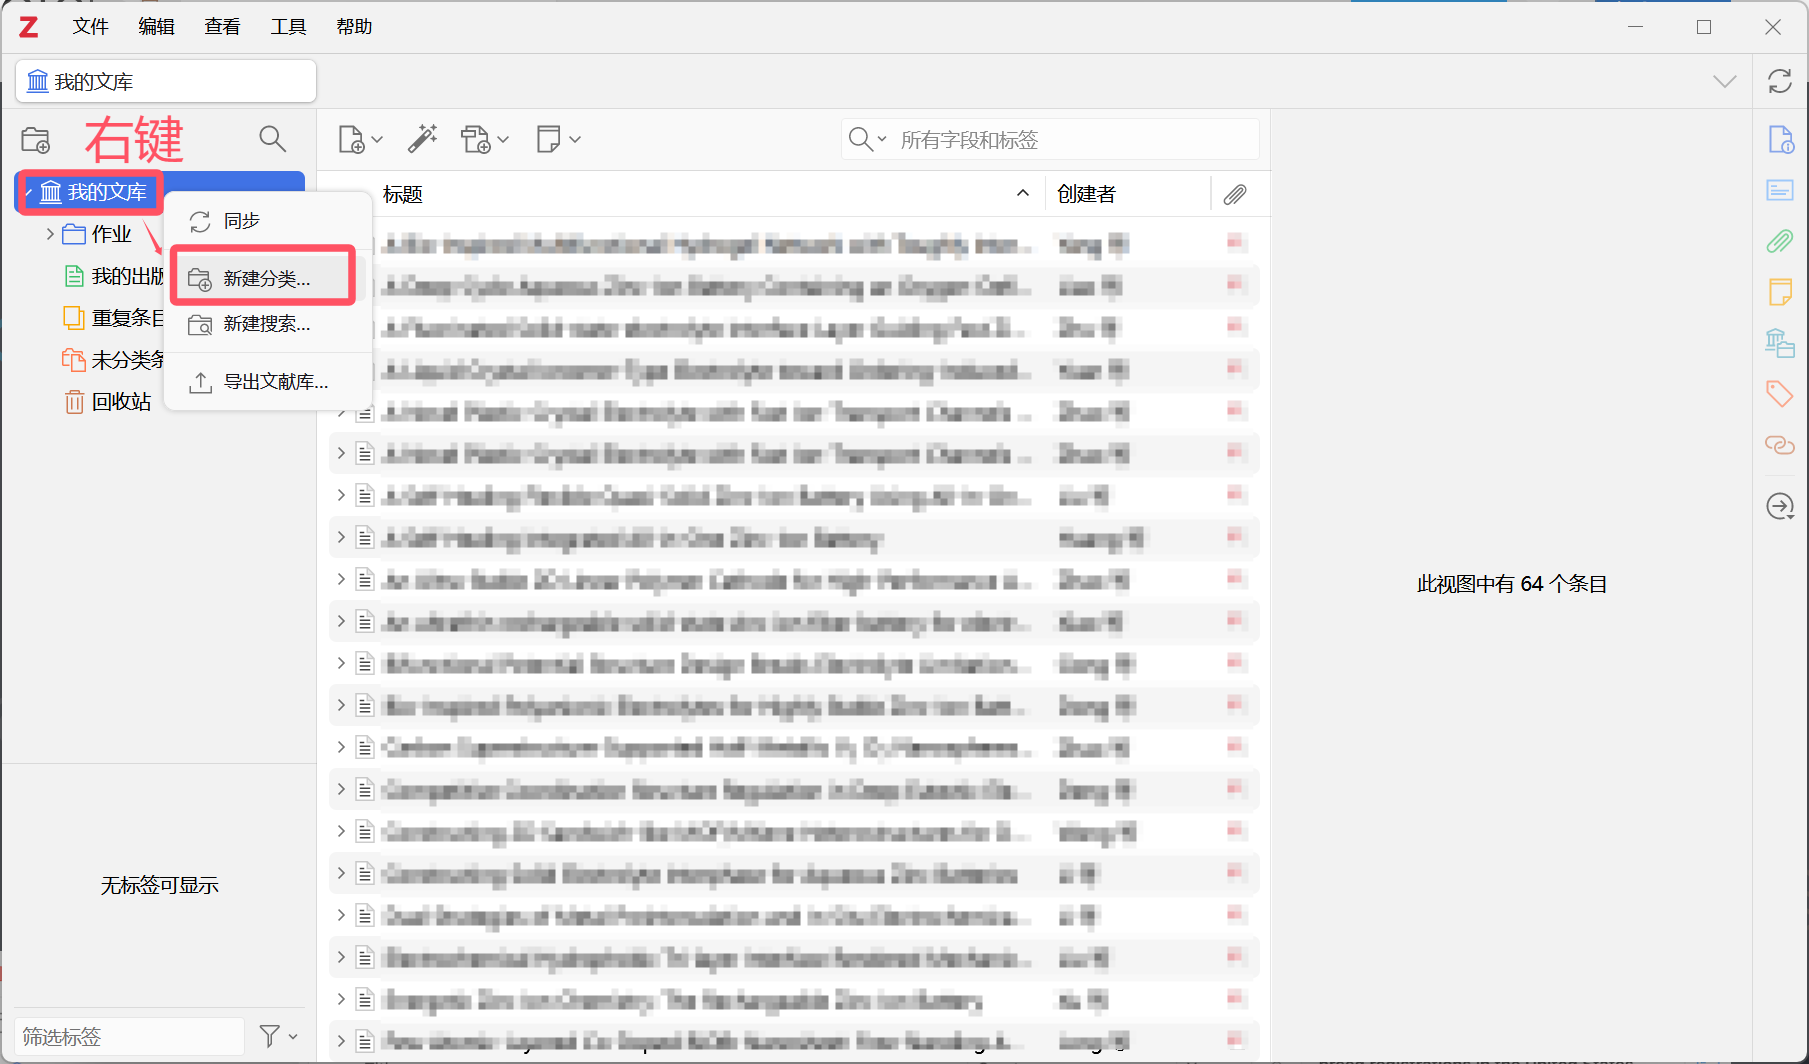
\includegraphics[width=0.8\textwidth]{Zotero打开.png}
    \caption{Zotero}
    \label{Zotero 1}
\end{figure}

\newpage

之后可直接拖拽文献PDF导入:

\begin{figure}[htbp]
    \centering
    \captionsetup{font={small, bf}, margin=60pt}
    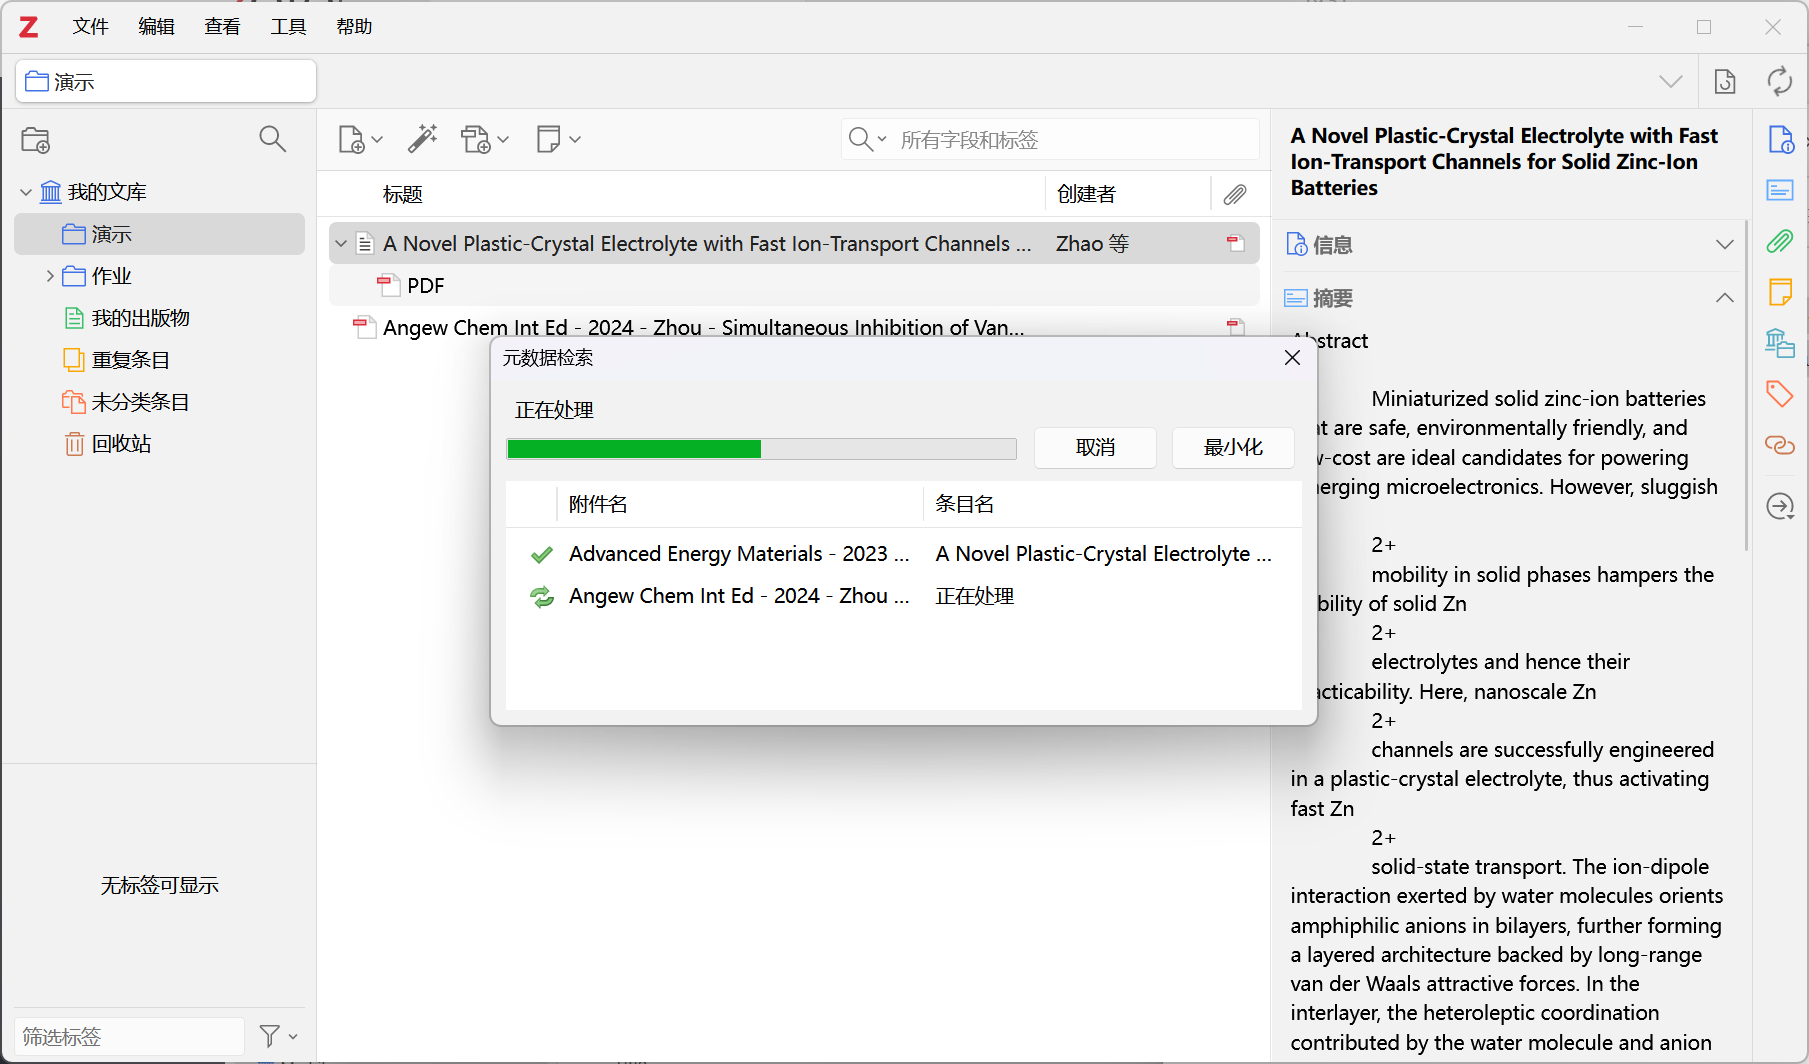
\includegraphics[width=0.8\textwidth]{Zotero导入.png}
    \caption{Zotero}
    \label{Zotero 2}
\end{figure}

也可以安装浏览器拓展直接在浏览器导入:
\begin{figure}[h]
    \centering
    \captionsetup{font={small, bf}, margin=60pt}
    \begin{subfigure}[c]{0.48\textwidth}
      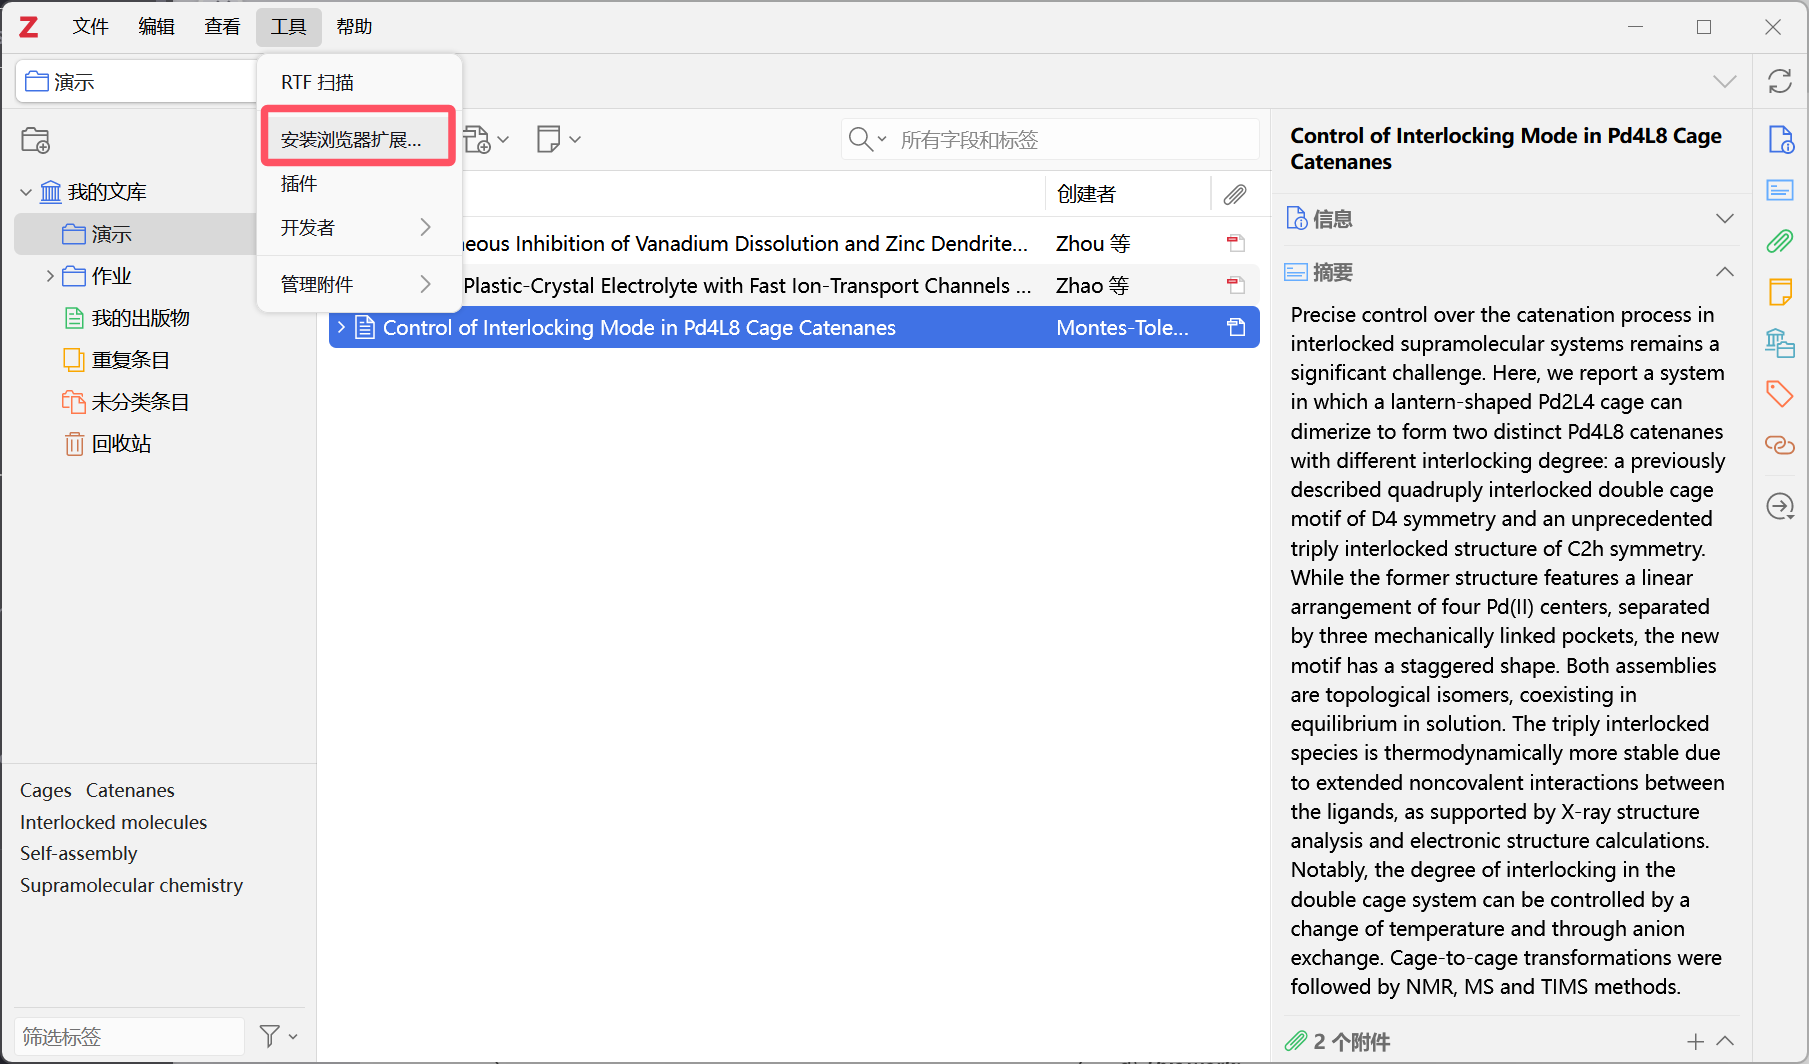
\includegraphics[width=\textwidth]{浏览器拓展安装.png}
      \label{Zotero 3-1}
    \end{subfigure}
    \hfill
    \begin{subfigure}[c]{0.48\textwidth}
      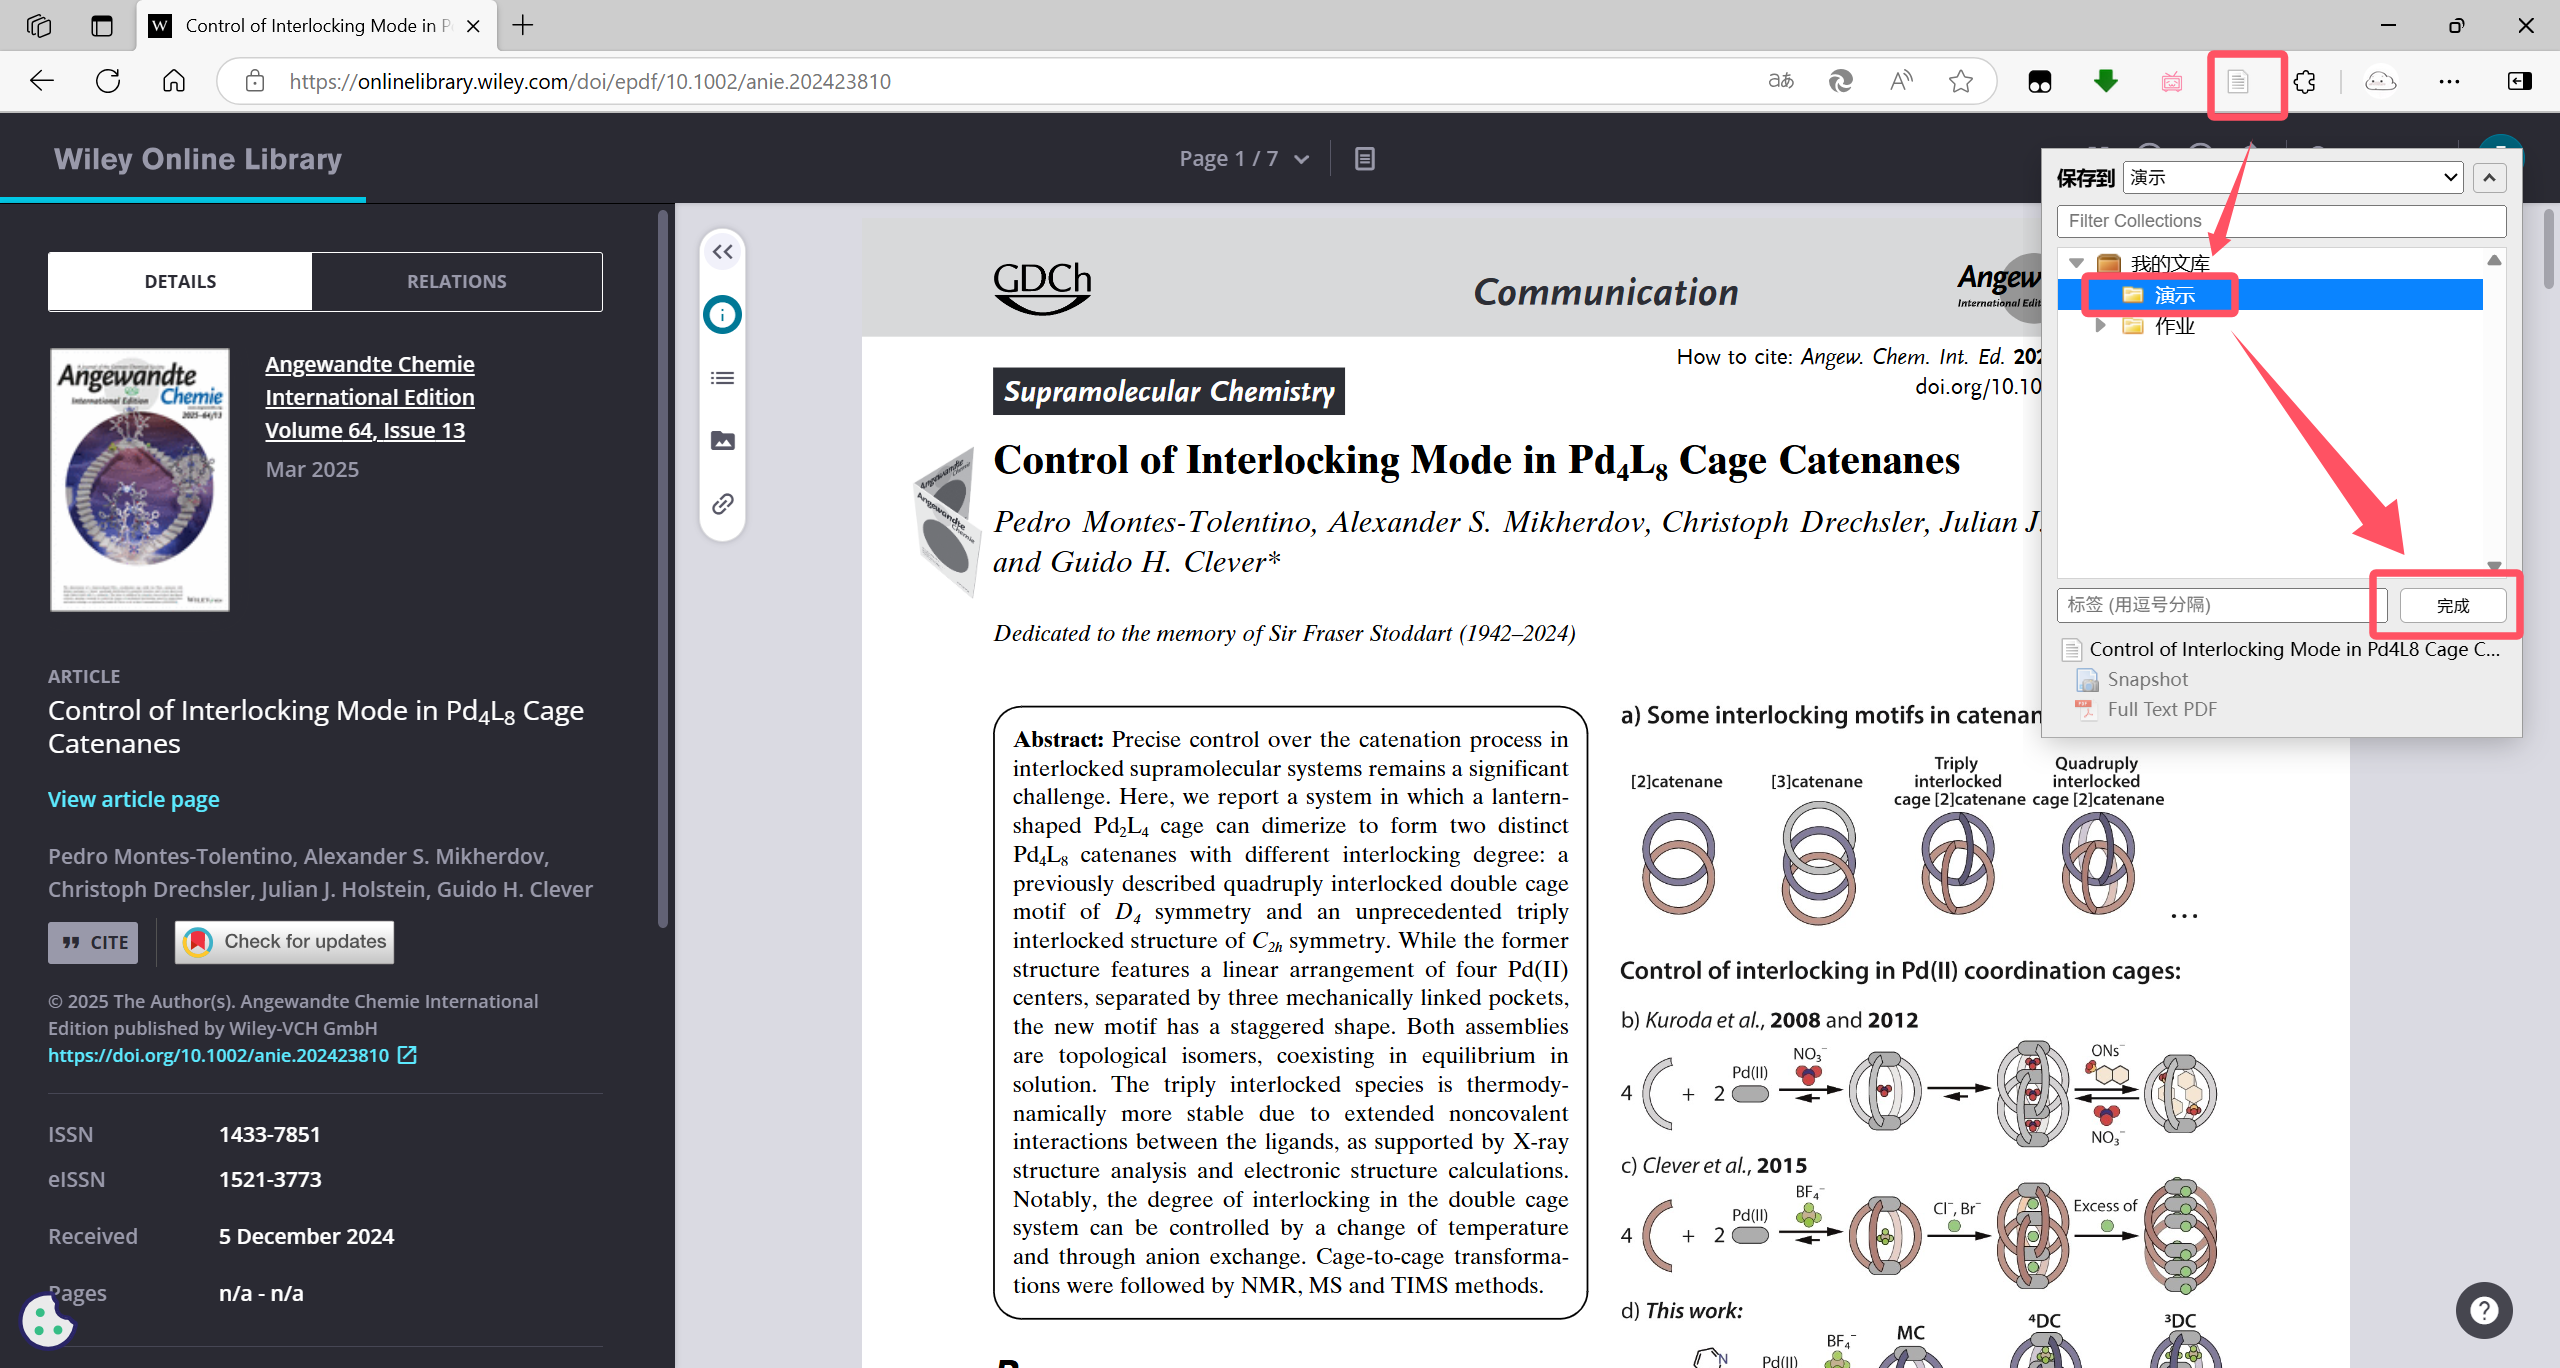
\includegraphics[width=\textwidth]{浏览器导入.png}
      \label{Zotero 3-2}
    \end{subfigure}
    \caption{直接在浏览器导入}
    \label{Zotero 3}
\end{figure}

Zotero具有强大的文献管理功能,配合一些插件也是不错的文献阅读软件。其它操作功能自行探索,不再赘述。

\newpage

\subsection{在Word中插入}
注:若需在其它地方(如PPT)插入参考文献,可在Zotero界面右击所需文件(可多选)或右击左侧文件夹,
选择“用所选条目创建参考文献表”,按提示选择样式,选择复制到剪贴板就可在所需地方粘贴。
但这种方式不如在Word中直接插入智能,不能自动排序或一键更新样式。

在Word中可以方便的使用Zotero插入参考文献,光标定位在要插入的地方,
点击上方Zotero选项卡,点击第一个“插入引用”,每一个文档中首次插入文献会询问引用样式,这个在下一节会讲到。
选择需要的样式后,切换到经典视图,即可插入文献:

\begin{figure}[h]
    \centering
    \captionsetup{font={small, bf}, margin=60pt}
    \begin{subfigure}[c]{0.48\textwidth}
      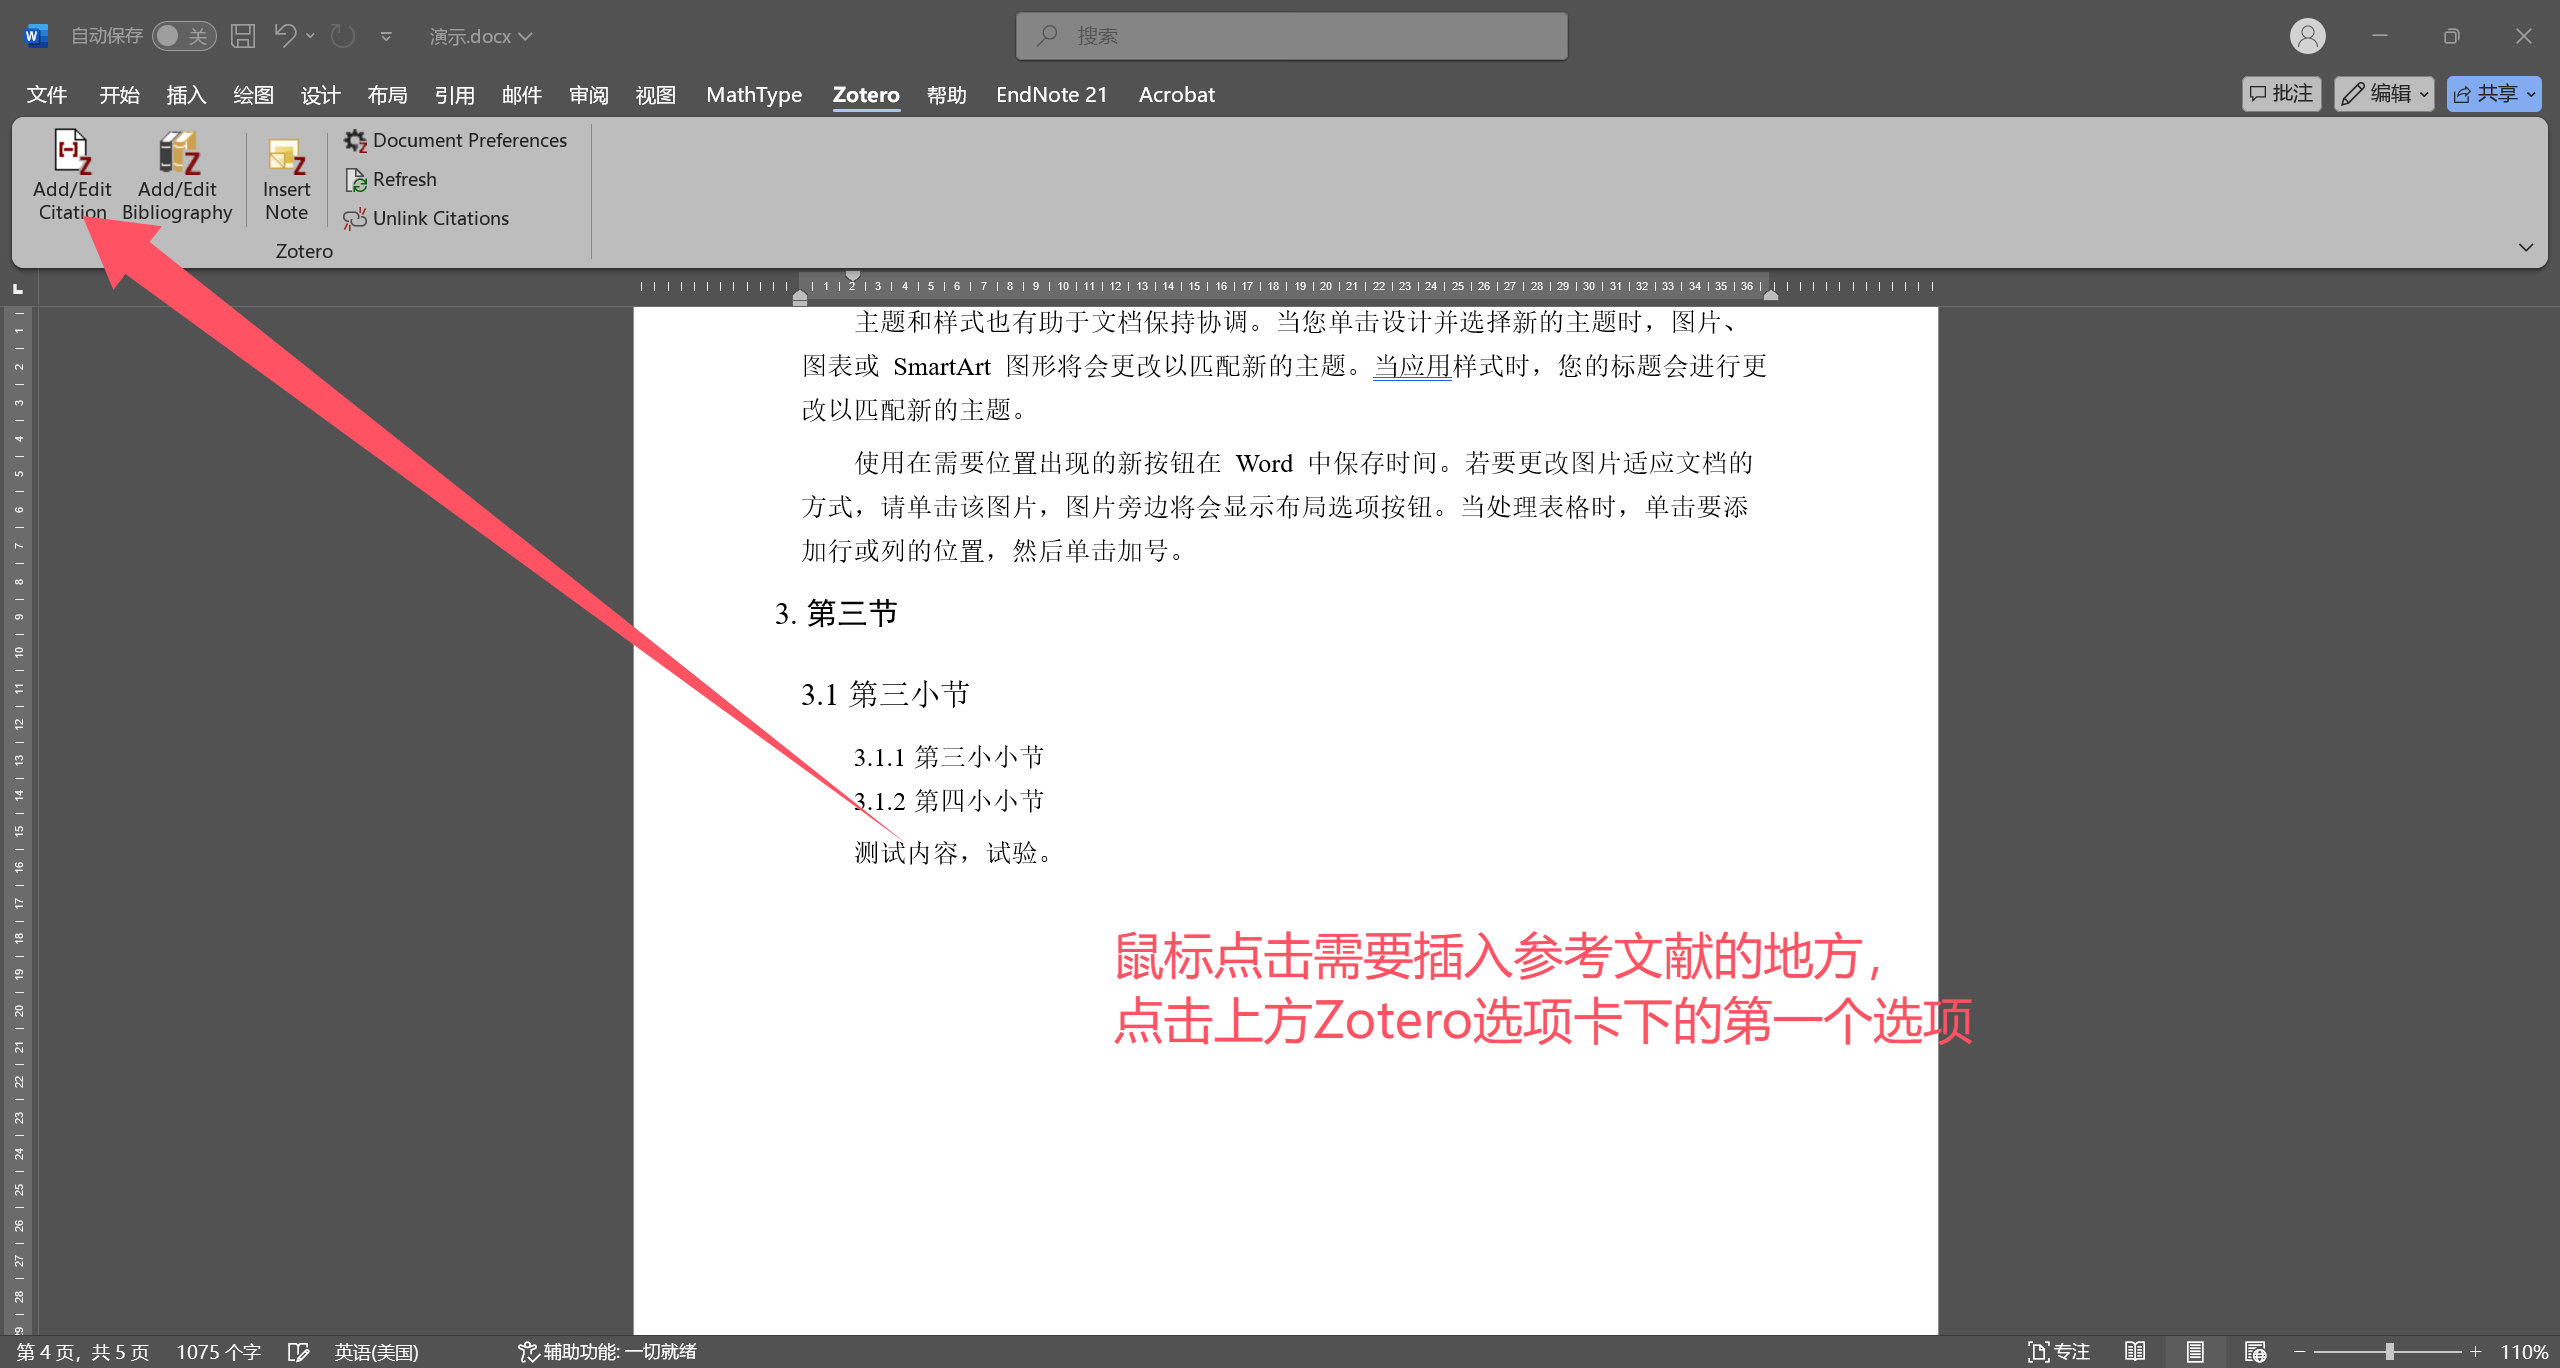
\includegraphics[width=\textwidth]{word使用Zotero-1.png}
      \label{Zotero 4-1}
    \end{subfigure}
    \hfill
    \begin{subfigure}[c]{0.48\textwidth}
      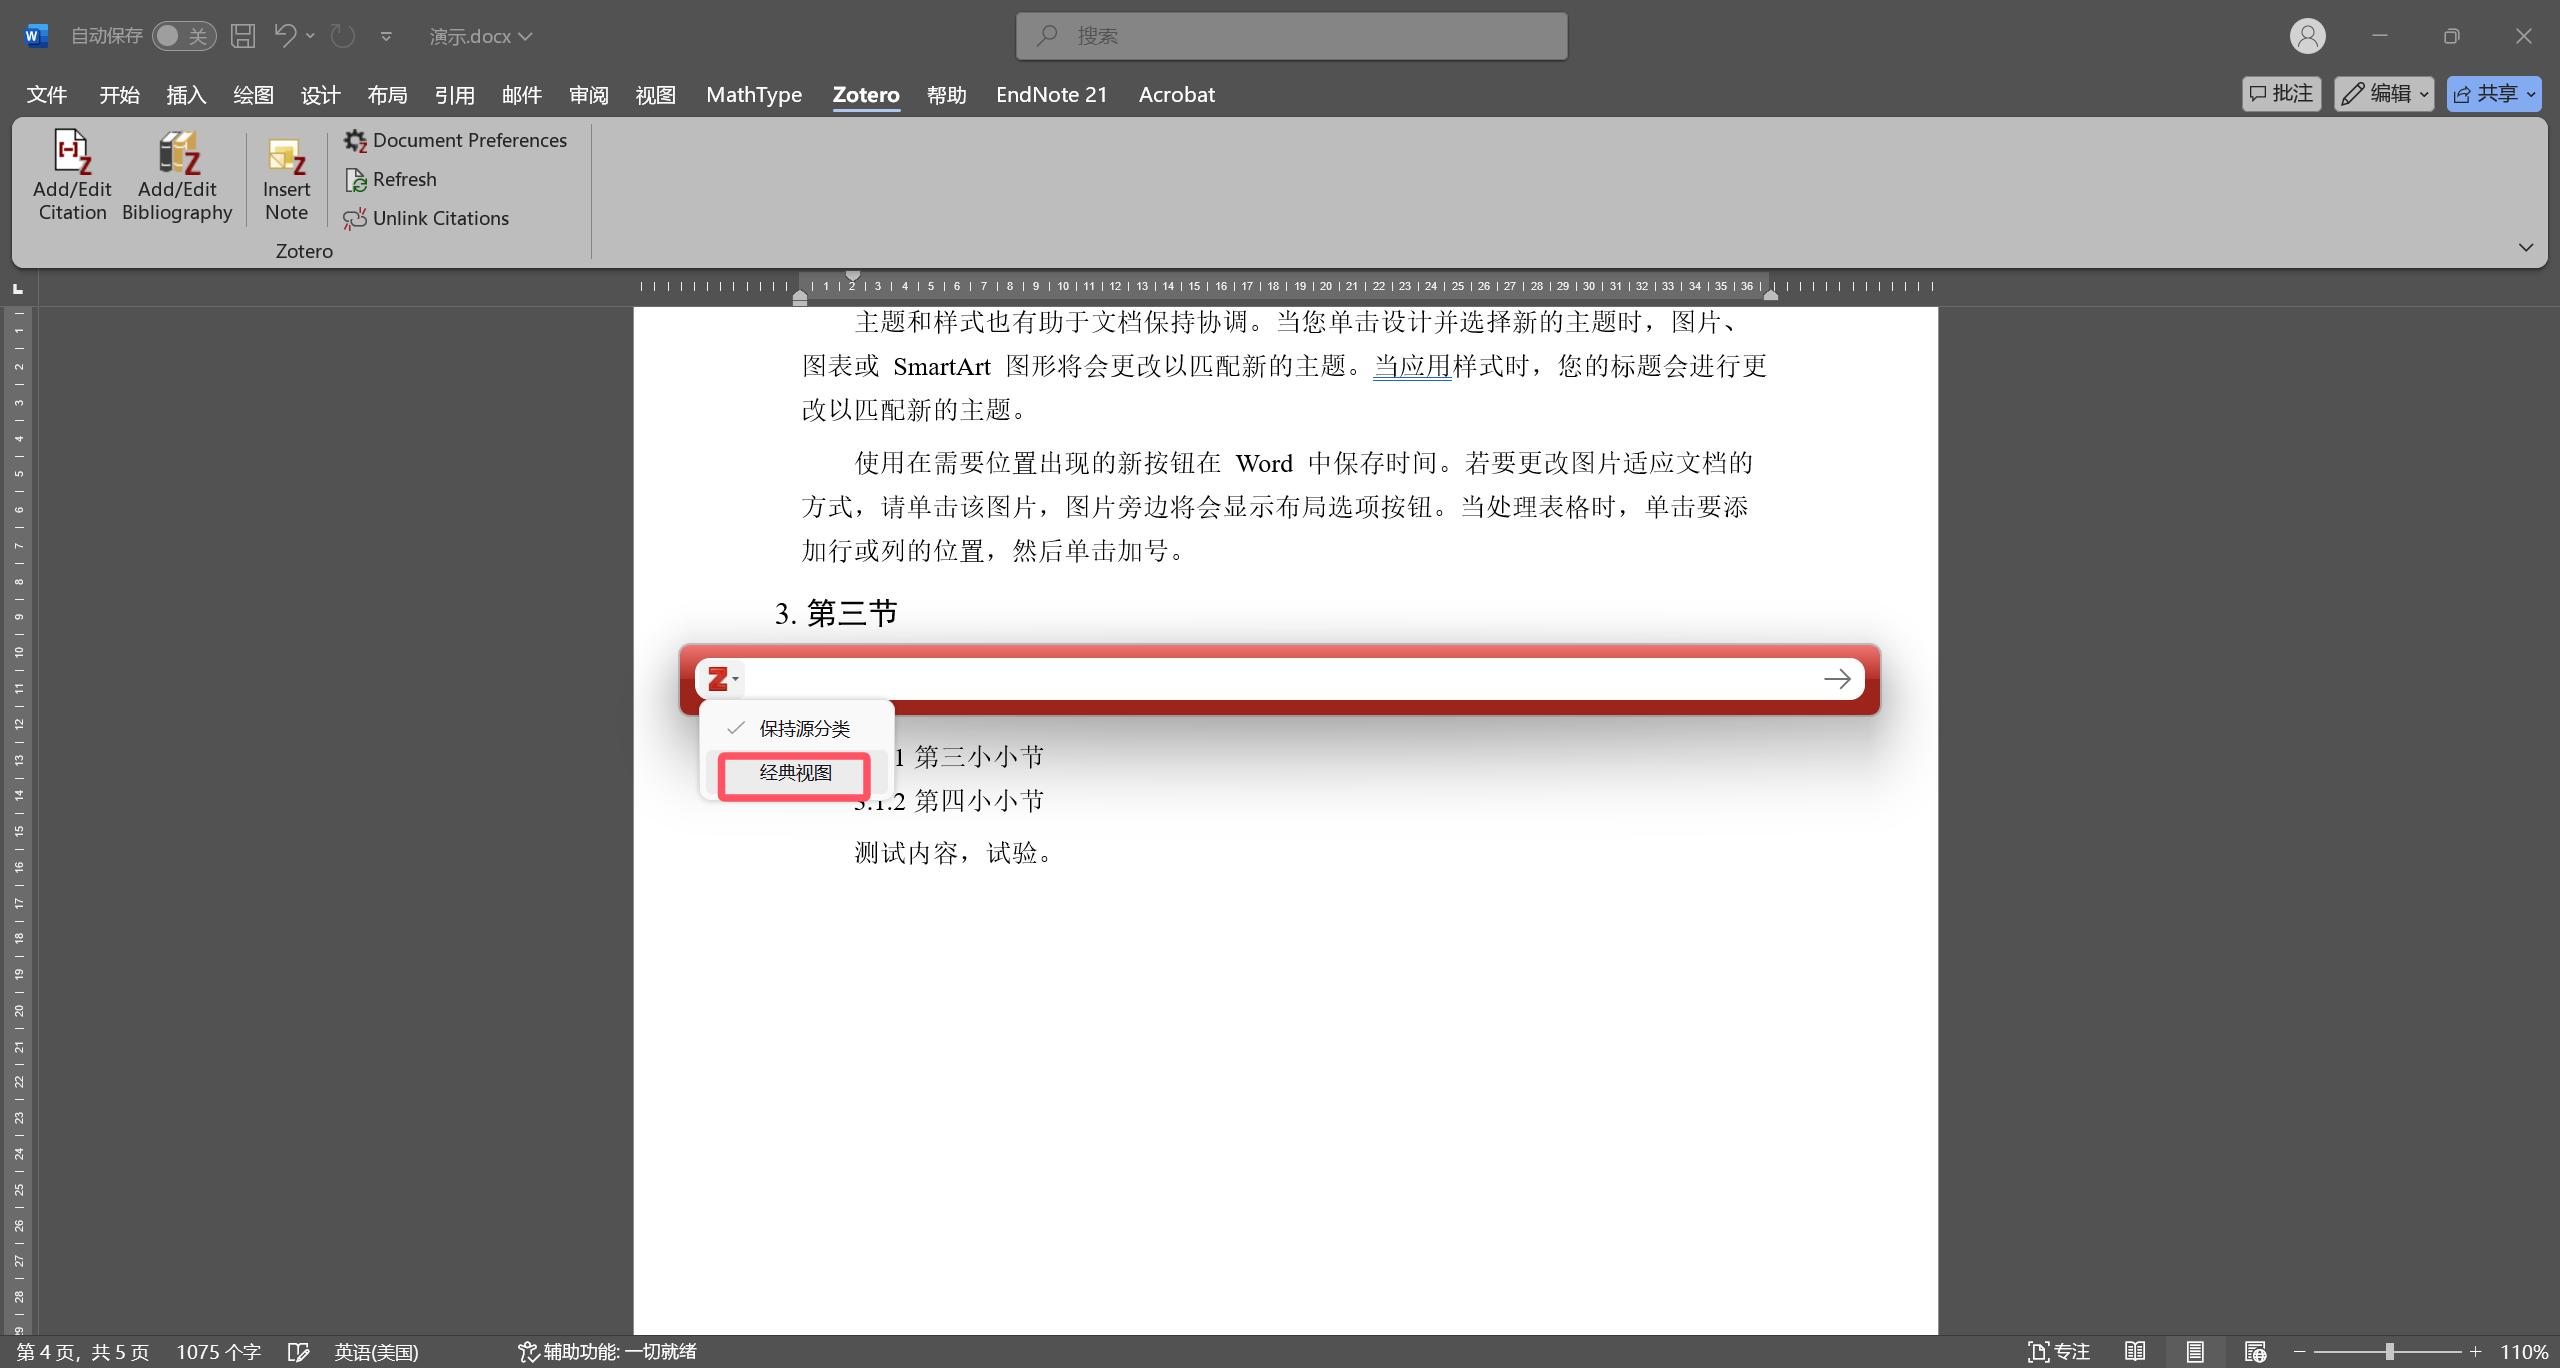
\includegraphics[width=\textwidth]{word使用Zotero-2.png}
      \label{Zotero 4-2}
    \end{subfigure}
    \hspace{-1em}
    \begin{subfigure}[c]{0.8\textwidth}
        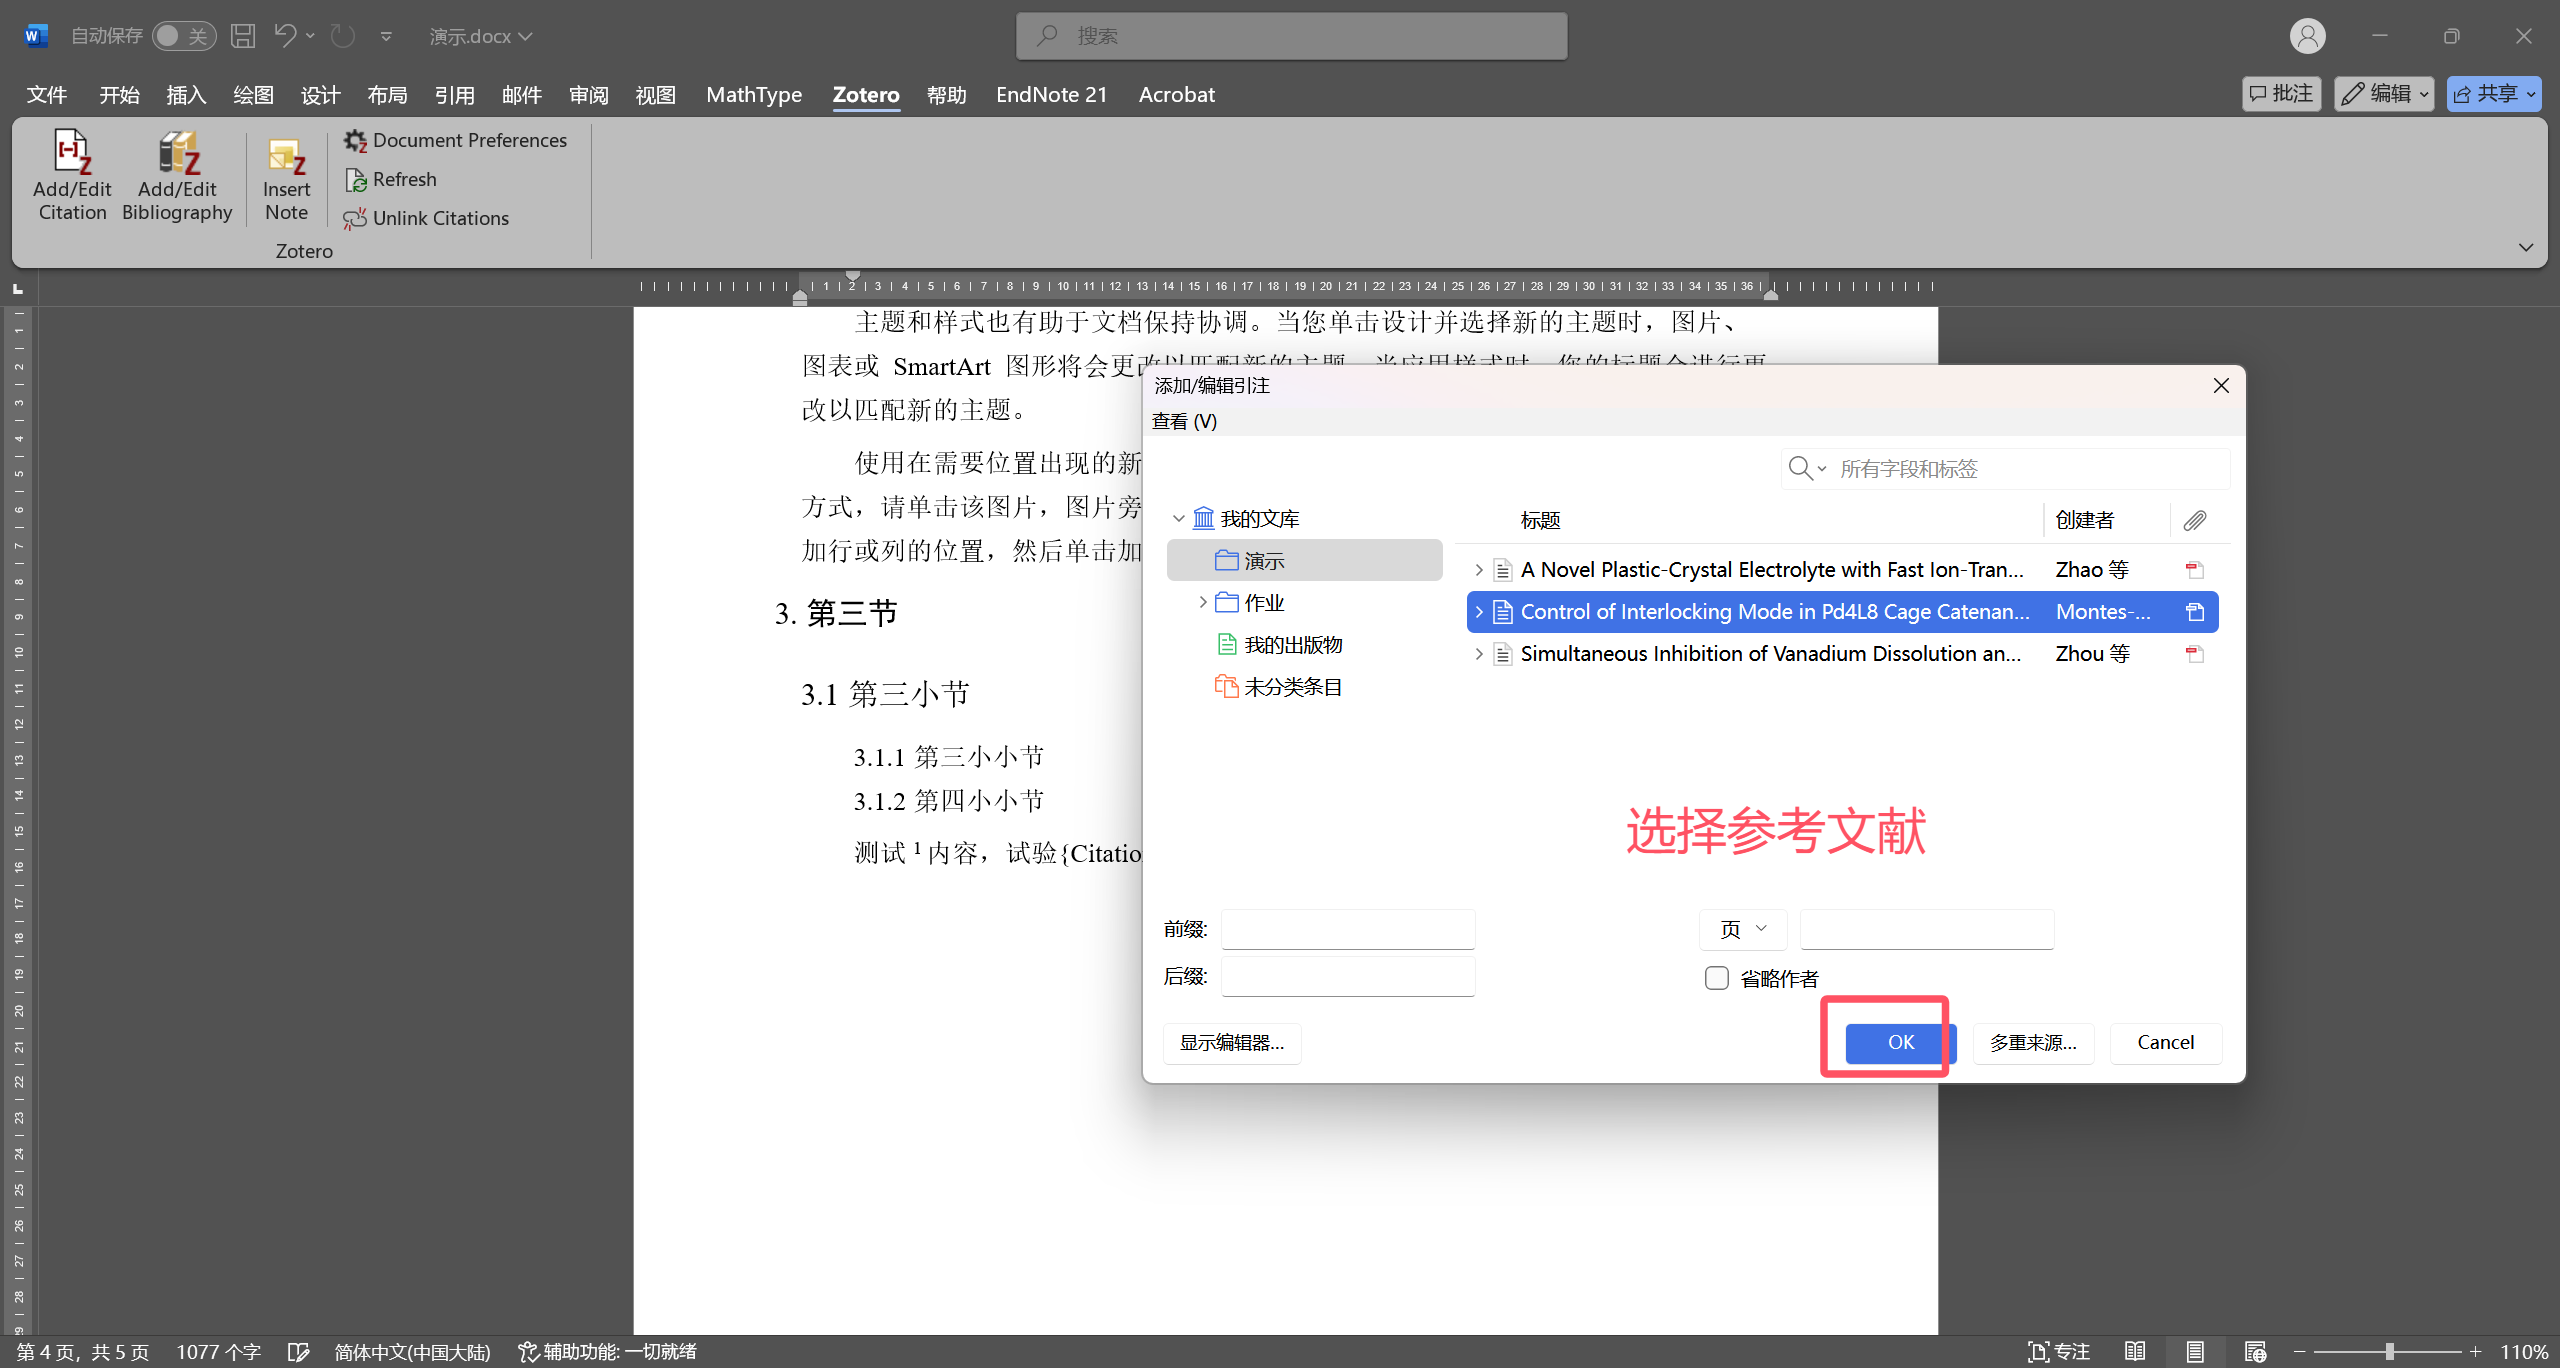
\includegraphics[width=\textwidth]{word使用Zotero-3.png}
        \label{Zotero 4-3}
    \end{subfigure}
    \caption{word使用Zotero}
    \label{Zotero 4}
\end{figure}

还可以插入多个文献,点击插入文献后,在经典视图下,选择“多个来源”,
选择要插入的文献,按右箭头图标进行选择,选择完成后按OK,即可插入:

\newpage

\begin{figure}[h]
    \centering
    \captionsetup{font={small, bf}, margin=60pt}
    \begin{subfigure}[c]{0.48\textwidth}
      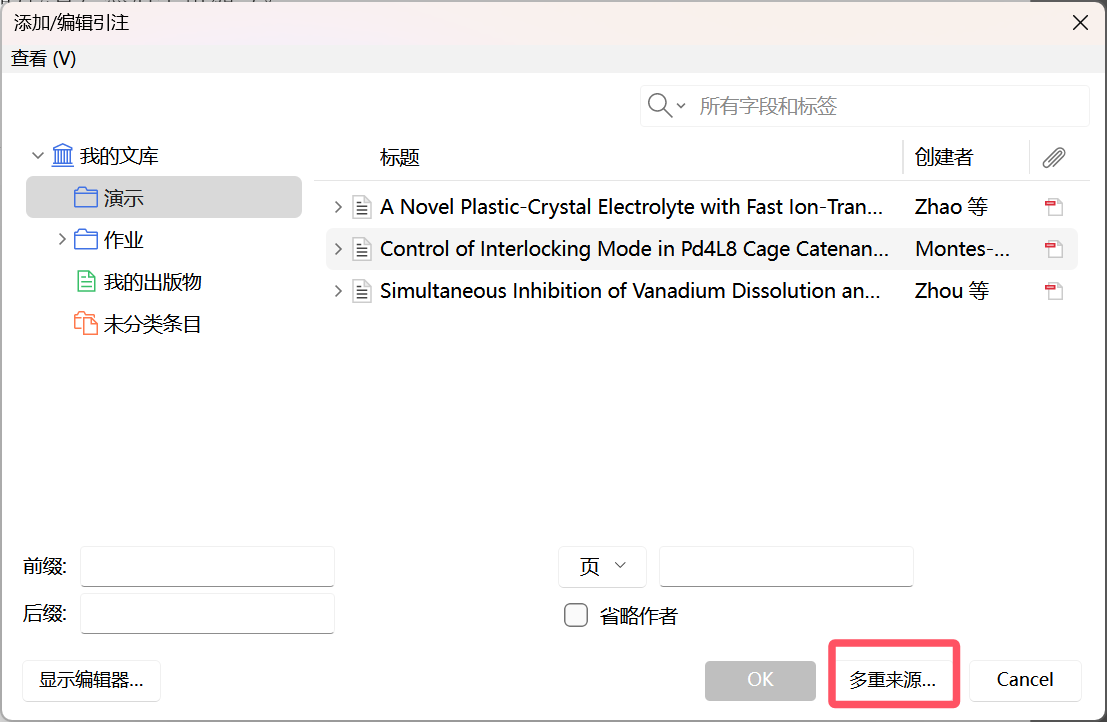
\includegraphics[width=\textwidth]{插入多个文献-2.png}
      \label{Zotero 5-1}
    \end{subfigure}
    \hfill
    \begin{subfigure}[c]{0.48\textwidth}
      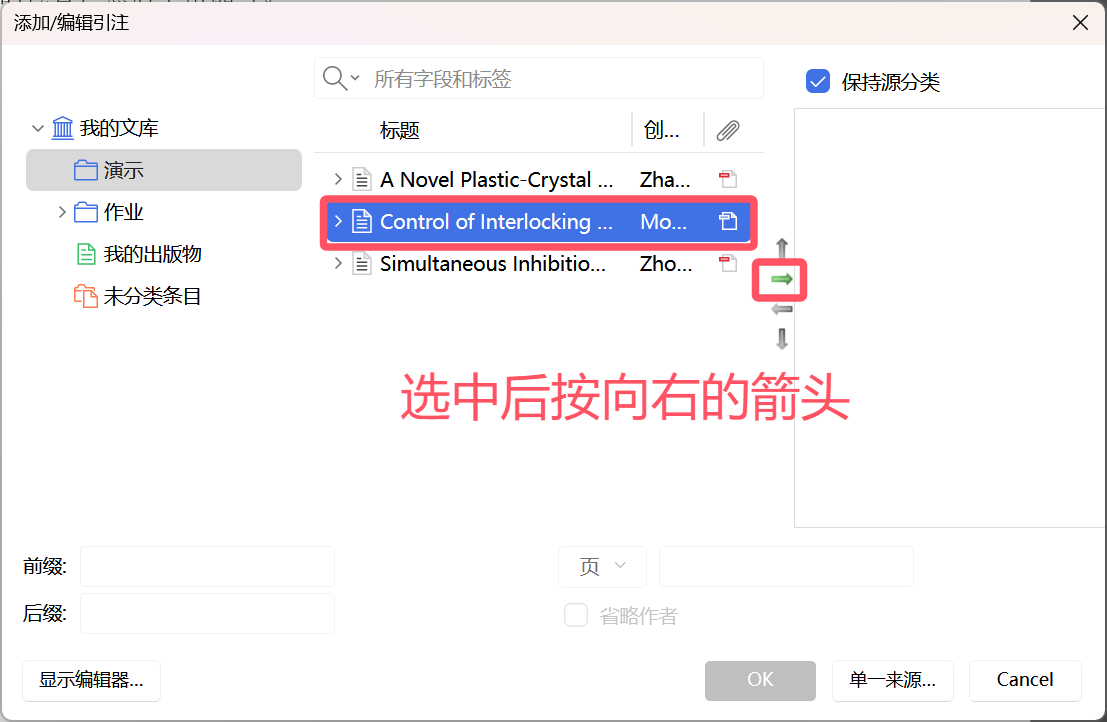
\includegraphics[width=\textwidth]{插入多个文献-1.png}
      \label{Zotero 5-2}
    \end{subfigure}
    \caption{插入多个文献}
    \label{Zotero 5}
\end{figure}

\begin{figure}[!h]
    \centering
    \captionsetup{font={small, bf}, margin=60pt}
    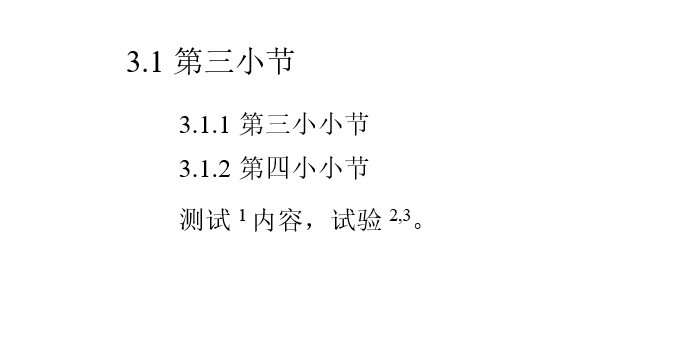
\includegraphics[width=0.6\textwidth]{插入多个文献效果.png}
    \caption{插入多个文献效果}
    \label{Zotero 6}
\end{figure}

随后在结尾直接点选“Zotero”选项卡下第二个选项“插入书目”,即可直接插入参考文献列表:
\begin{figure}[!h]
    \centering
    \captionsetup{font={small, bf}, margin=60pt}
    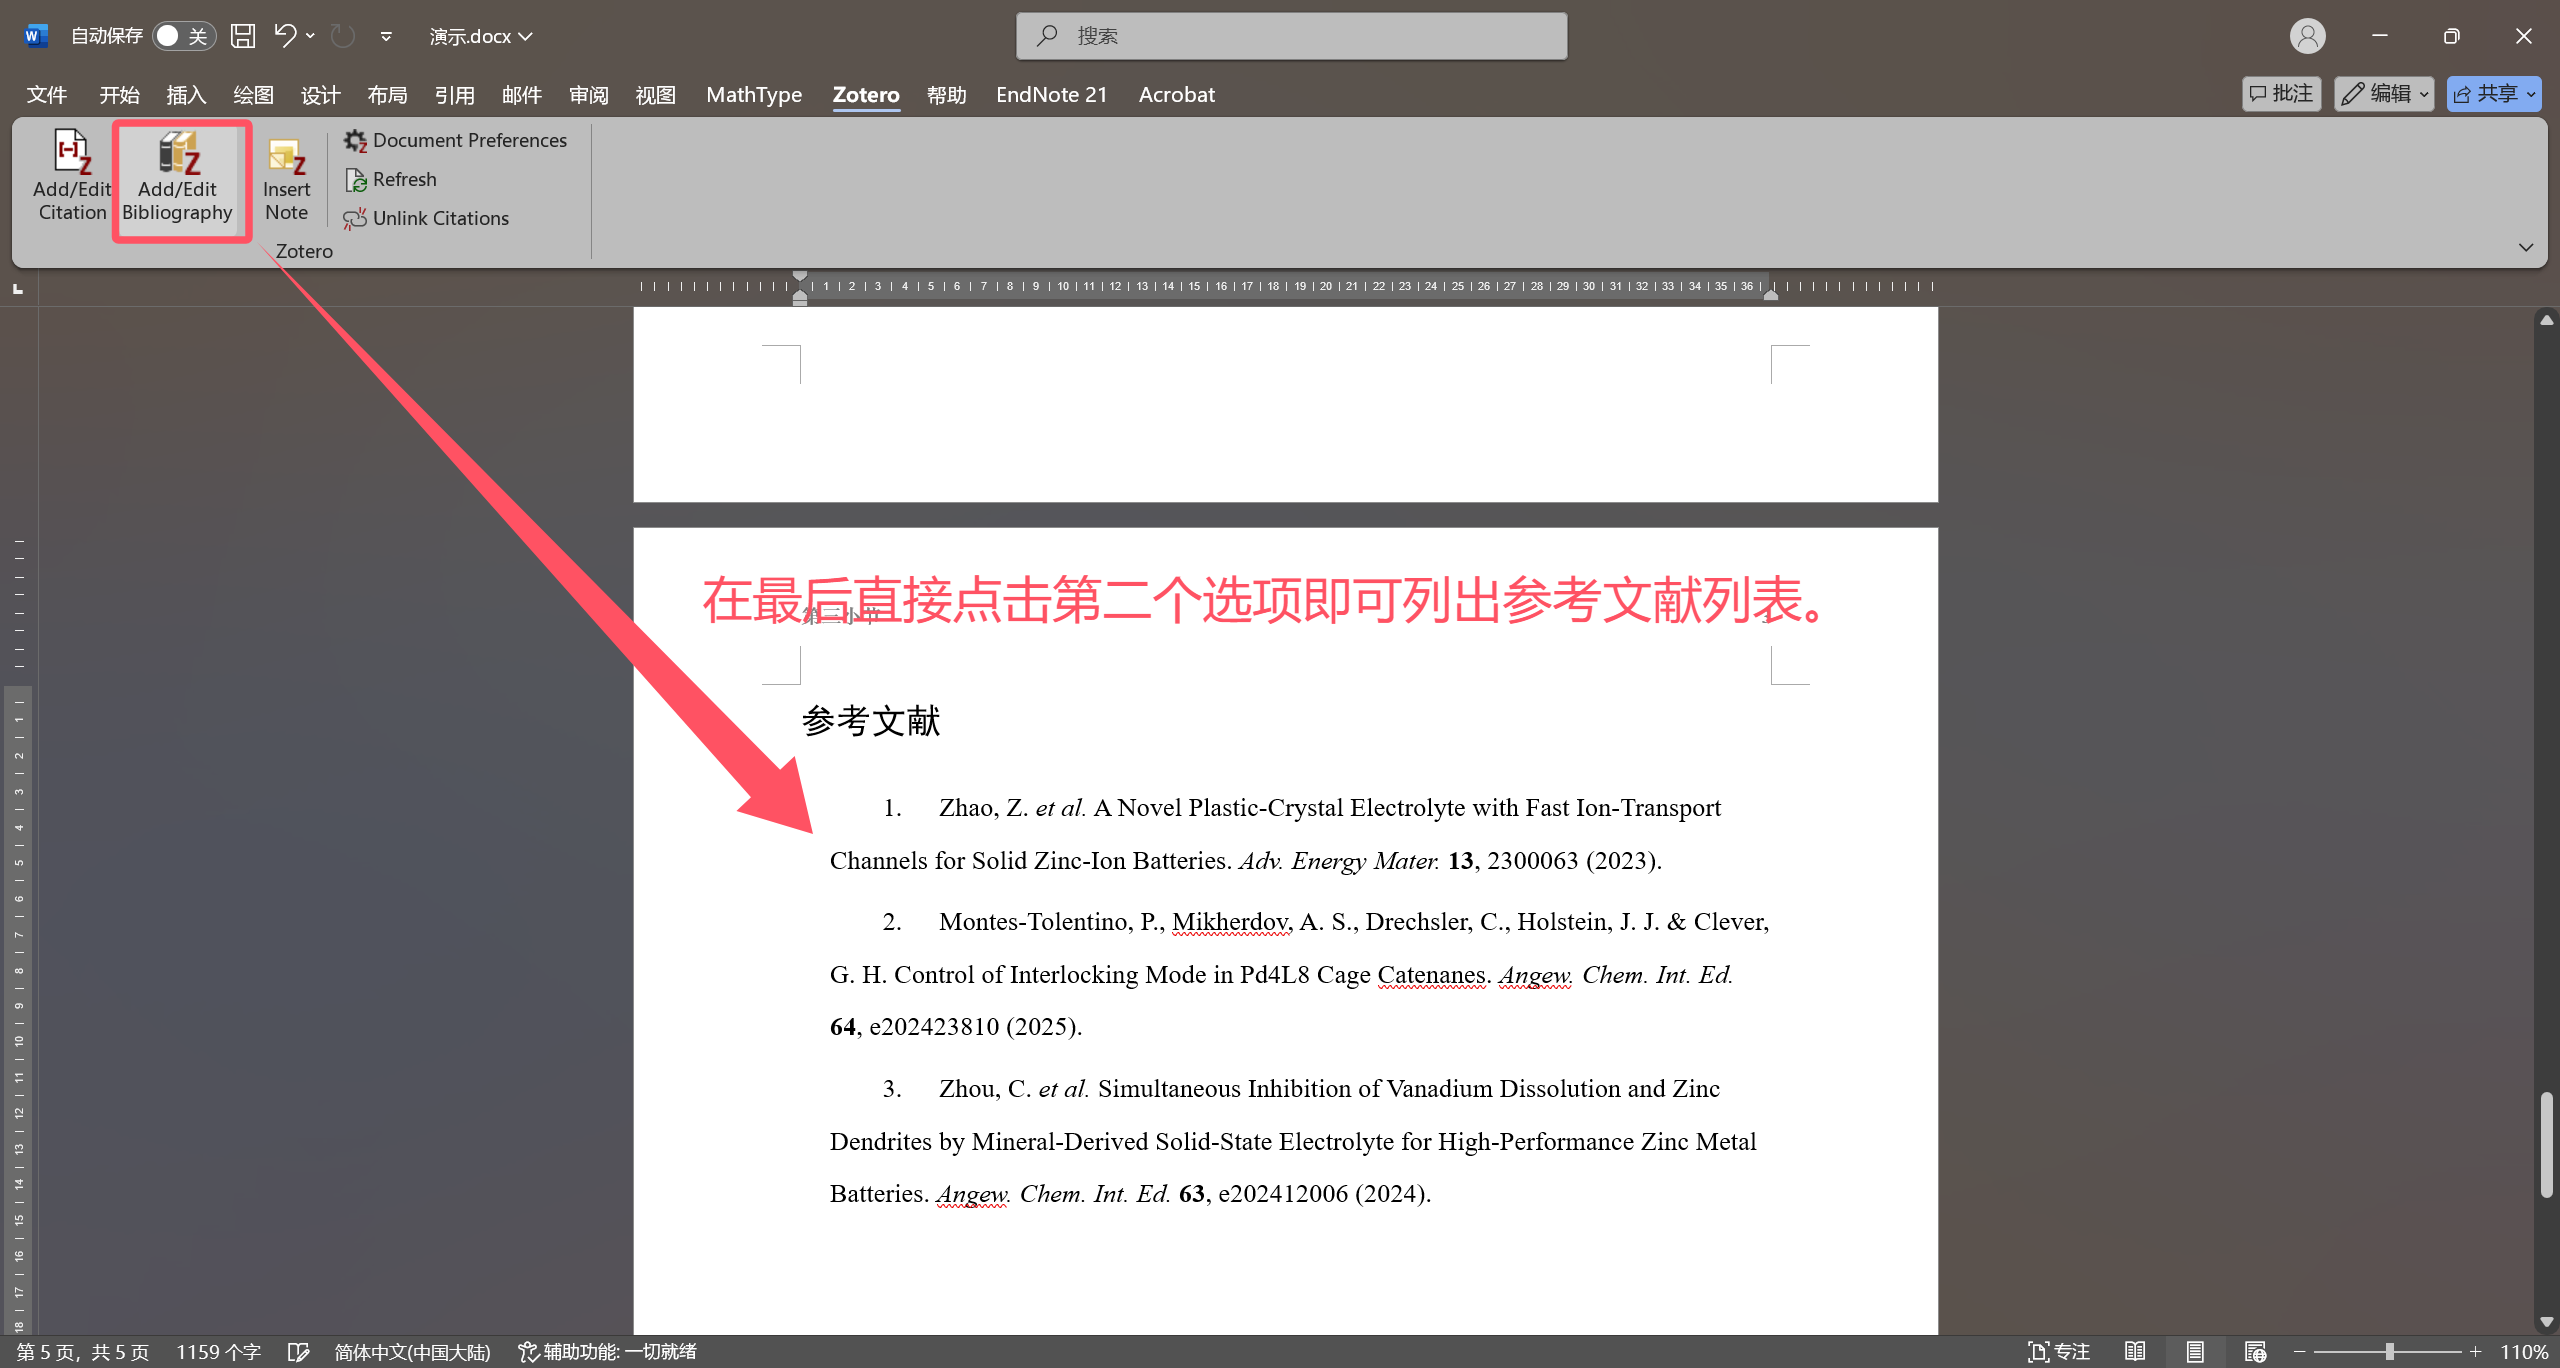
\includegraphics[width=0.6\textwidth]{参考文献.png}
    \caption{参考文献}
    \label{Zotero 7}
\end{figure}

\subsection{参考文献样式}
\subsubsection{选定及更改参考文献样式}
如上节提到,每个Word文档在首次插入文献时会询问参考文献样式,
选择之后,如需更改,可在“Zotero”选项卡下的“Document Preferences”中更改,
若没有立即生效,可点点击“Refresh”手动刷新。
\begin{figure}[!h]
    \centering
    \captionsetup{font={small, bf}, margin=60pt}
    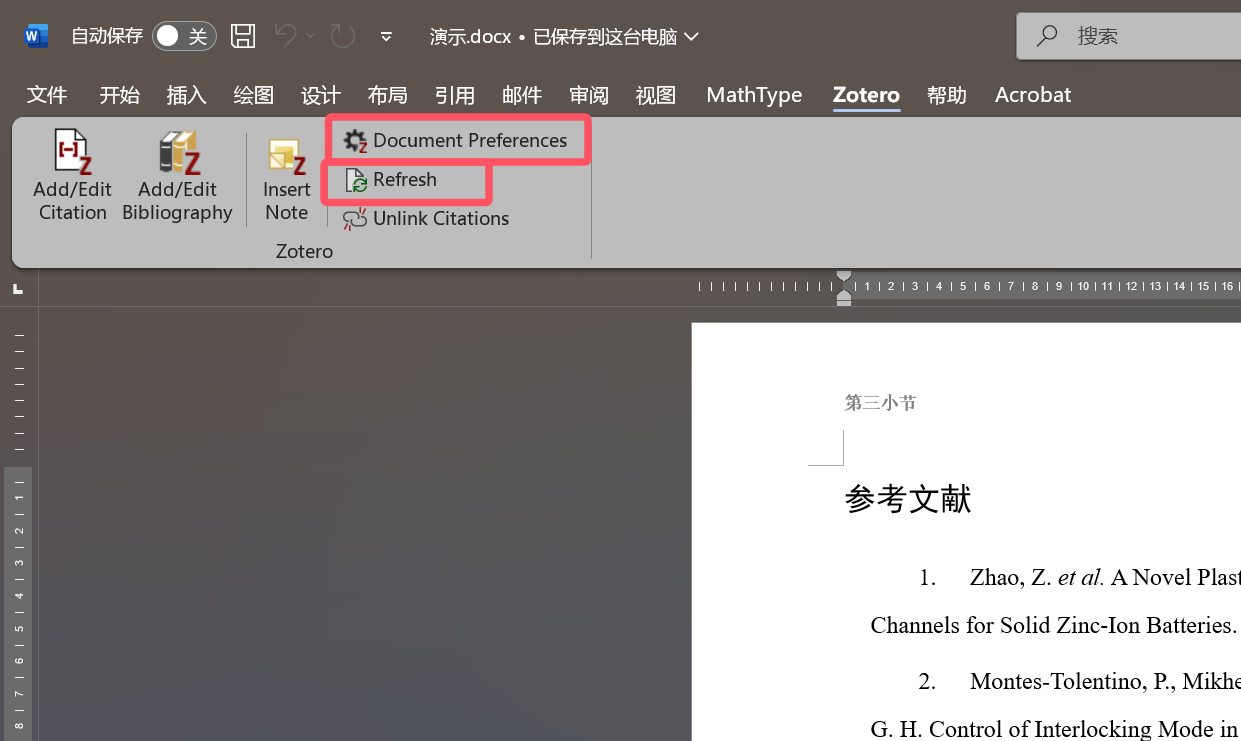
\includegraphics[width=0.6\textwidth]{参考文献样式-1.png}
    \caption{参考文献样式}
    \label{Zotero 8}
\end{figure}

\subsubsection{国标样式}
在国内,我们常用GB/T 7714-2015国标格式,Zotero中需要手动下载。
但在软件内下载的样式有一些缺陷,对双语不友好。
如作者为英文或拼音时,姓名会全部大写,且省略过多作者时显示“等”而不是“et al.”。
针对这些问题,有人整理了更好用的样式,这里提供给大家,可按下图所示安装:

\begin{figure}[!h]
  \centering
  \captionsetup{font={small, bf}, margin=60pt}
  \begin{subfigure}[c]{0.9\textwidth}
      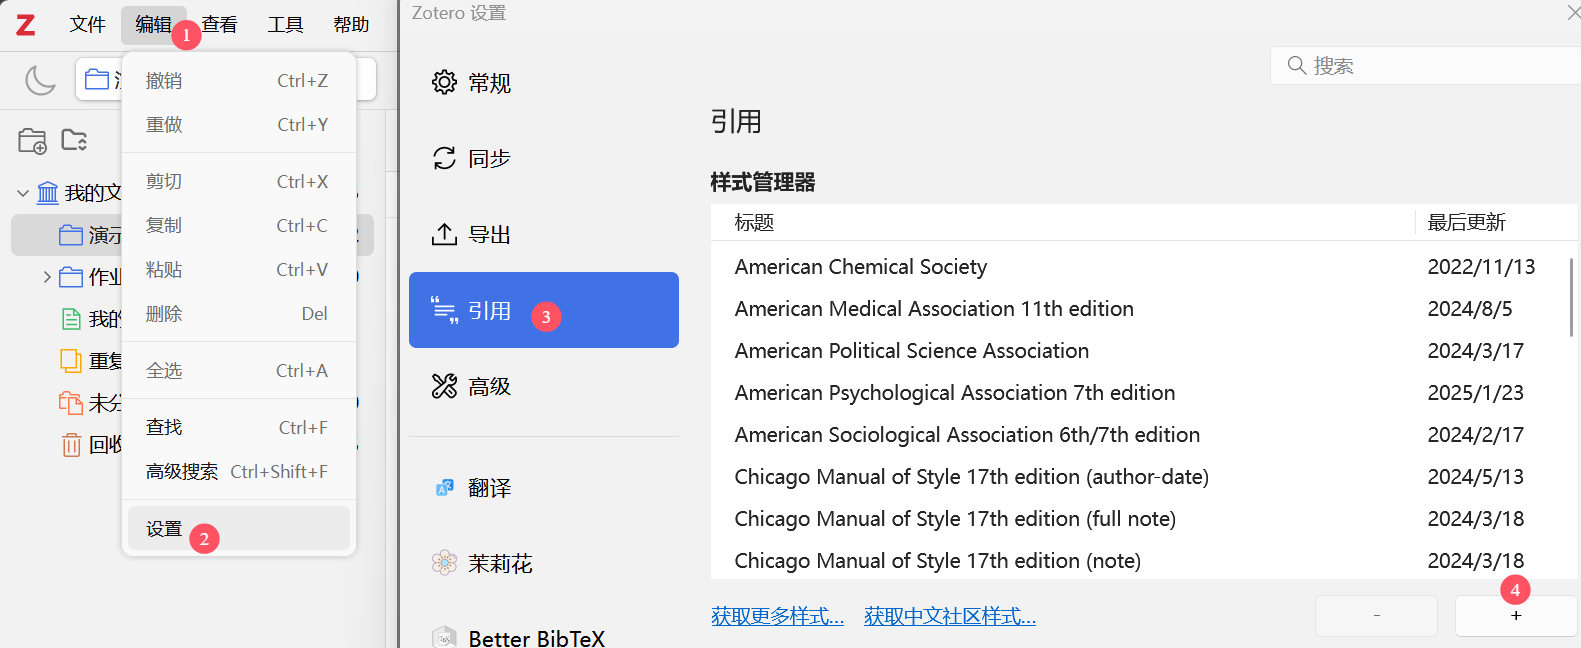
\includegraphics[width=\textwidth]{安装样式-1.png}
      \label{Zotero 9}
  \end{subfigure}
\end{figure}
  \hspace{-1em}

\begin{figure}[h]
  \centering
  \captionsetup{font={small, bf}, margin=60pt}
  \begin{subfigure}[c]{0.48\textwidth}
    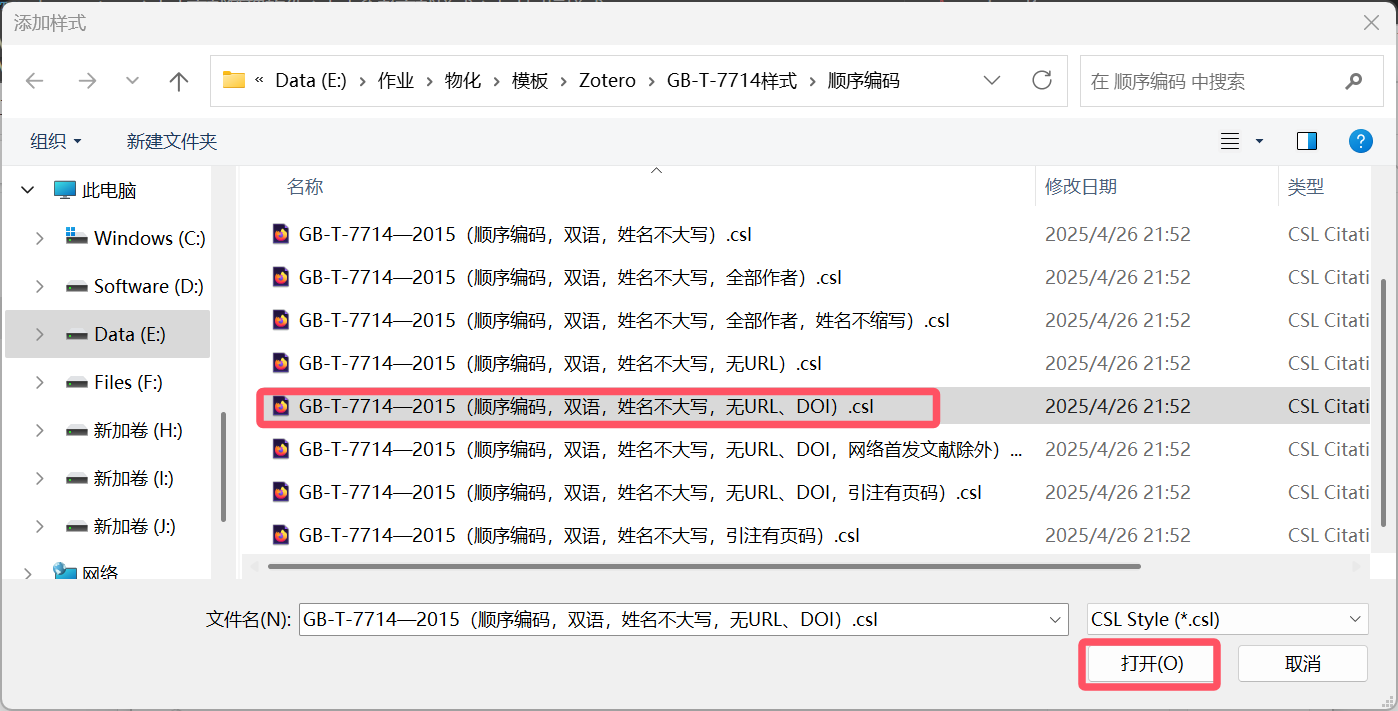
\includegraphics[width=\textwidth]{安装样式-2.png}
    \label{Zotero 10-1}
  \end{subfigure}
  \begin{subfigure}[c]{0.48\textwidth}
    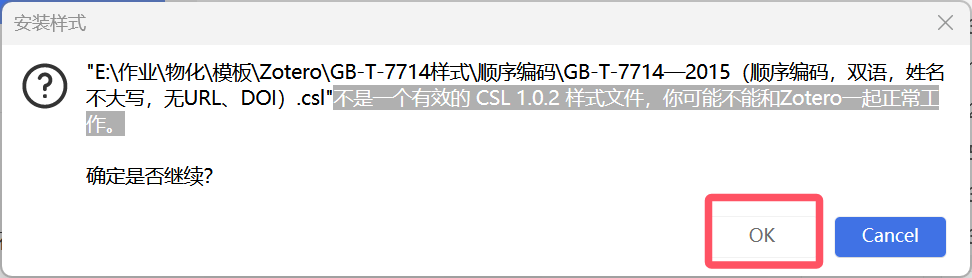
\includegraphics[width=\textwidth]{安装样式-3.png}
    \label{Zotero 10-2}
  \end{subfigure}
  \caption{安装样式}
  \label{Zotero 10}
\end{figure}

我们一般就使用“顺序编码,双语,姓名不大写,无URL、DOI”,其它样式可以按需取用。
安装完成之后,就可以在“Document Preferences”中选择对应样式使用了。

\subsection{插件}
Zotero拥有丰富的插件生态,这里提供两个插件,一个是翻译,在Zotero中查看PDF时,
可以选中文字自动翻译;另一个是茉莉花插件,提供中文文献支持。按如下步骤安装:
\begin{figure}[h]
  \centering
  \captionsetup{font={small, bf}, margin=60pt}
  \begin{subfigure}[c]{0.48\textwidth}
    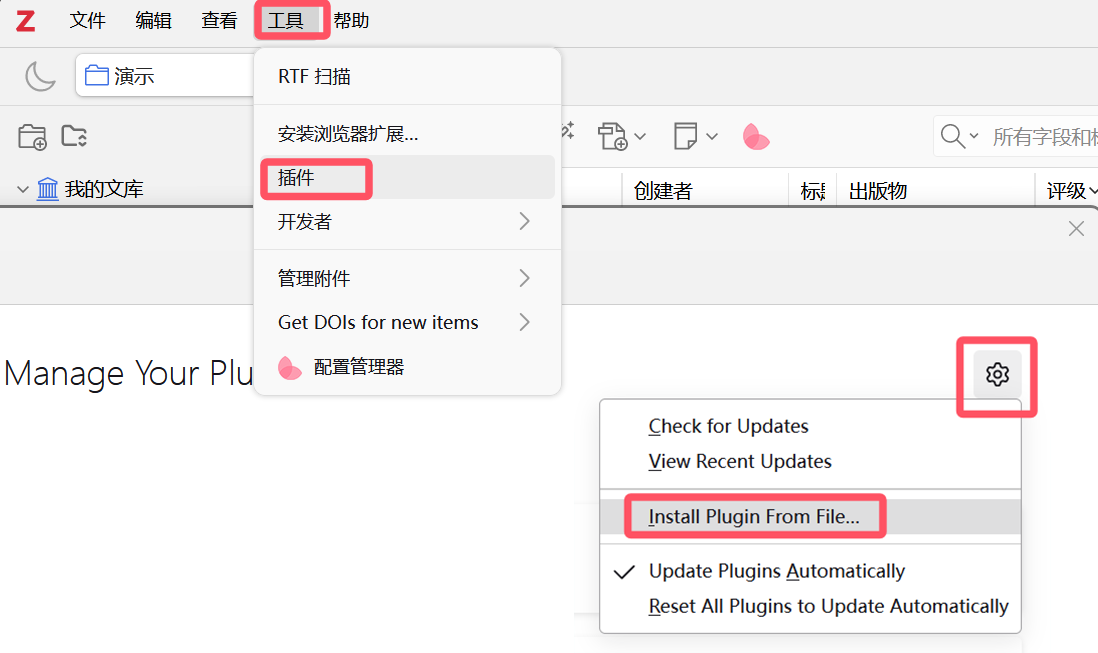
\includegraphics[width=\textwidth]{插件-1.png}
   \label{Zotero 11-1}
  \end{subfigure}
  \hfill
  \begin{subfigure}[c]{0.48\textwidth}
    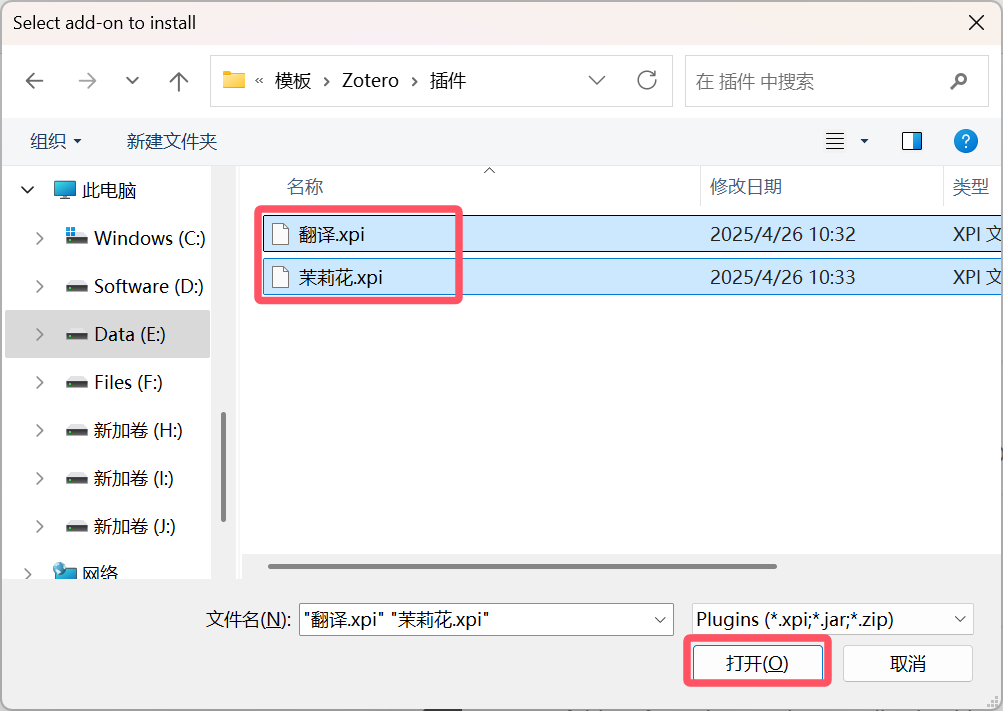
\includegraphics[width=\textwidth]{插件-2.png}
    \label{Zotero 11-2}
  \end{subfigure}
  \caption{插件}
  \label{Zotero 11}
\end{figure}

其他插件可以在\textbf{\textcolor{blue}{\href{https://zotero-chinese.com/plugins/}{Zotero中文社区插件}}}找到,安装方法类似。

\newpage
\section{Word相关操作}
\subsection{公式排版相关知识}
在数学上,一般规定,字母(包括角标上的字母)作为变量时用斜体,不是变量时用直立体(正体)。

比如$x^2+x+1=0$这里三个字母都是变量,就都是斜体。$x=\frac{-1\pm{}\sqrt{3}\mathrm{i}}{2}$中$\mathrm{i}$不是变量,用直立体。
另外,自然常数$\mathrm{e}$和圆周率$\uppi$还有微分符号$\mathrm{d}$都不是变量,用直立体。以及热力学中$\Delta{}T_{ab}$的角标表示的是a点和b点,也不是变量,用直立体,这里的$\Delta$也是直立体。

除此之外,在数学规定的基础上,热力学中状态函数和相关物理量如$H$、$G$、$S$、$T$、$P$、$V$、$n$等都用斜体。在化学分子式中,字母和数字都是直立体。

Word的公式编辑器会默认所有字体全都是斜体的,有时候需要自己手动更改为直立体。

\subsection{WPS}
\subsubsection{WPS优缺点}
尽量不要使用WPS!!!很多时候WPS会造成莫名其妙的混乱,请尽量不要使用。

WPS可能有很多内置模板,方便使用。并且学校也购买了正版,可以直接使用。
另外,WPS提供教育版,免费无广告,也可下载使用。

如果只是个人使用,无需与其他人交互,不向外共享文件,或转换成PDF共享,
幻灯片也只在自己电脑上放映,WPS还是不错的。
但是很多时候都会遇到兼容性问题。
特别是专业领域,如插入数学公式,或者ChemDraw图形,WPS很难胜任。

\subsubsection{使用MS Office} 

另外如果你购买的是带有系统的品牌电脑,售价的一部分是包括MS Office家庭版的,
可以直接打开使用,并无需付费。
如果你的品牌机赠送的是Office365一年或两年订阅,使用期过后,
也可到\textbf{\textcolor{blue}{\href{https://zbhrj1.jlu.edu.cn/download/office2021.html}{吉大正版网站}}}下载使用。

\subsection{Word模板使用}
\textbf{此部分请自行操作体会}:
Word模板文件通常以.dotx为后缀,双击即可新建文档。\textbf{注意}此时是新建文档,
并不是编辑模板文件,只是以模板文件为基础新建一个文档。
\textbf{可先另存为到本地,之后再进行编辑。}

\subsection{Word标题格式}

我提供的模板文件中已经设置了标题格式,直接使用即可。
另外,\textbf{标题无需手动编号},已设置自动编号:

\begin{figure*}[!h]
    \captionsetup{font={small, bf}, margin=60pt}
    \centering
    
\includegraphics[width=\textwidth]{模板标题.png}
\end{figure*}
\begin{figure}[!h]
    \captionsetup{font={small, bf}, margin=60pt}
    \centering
    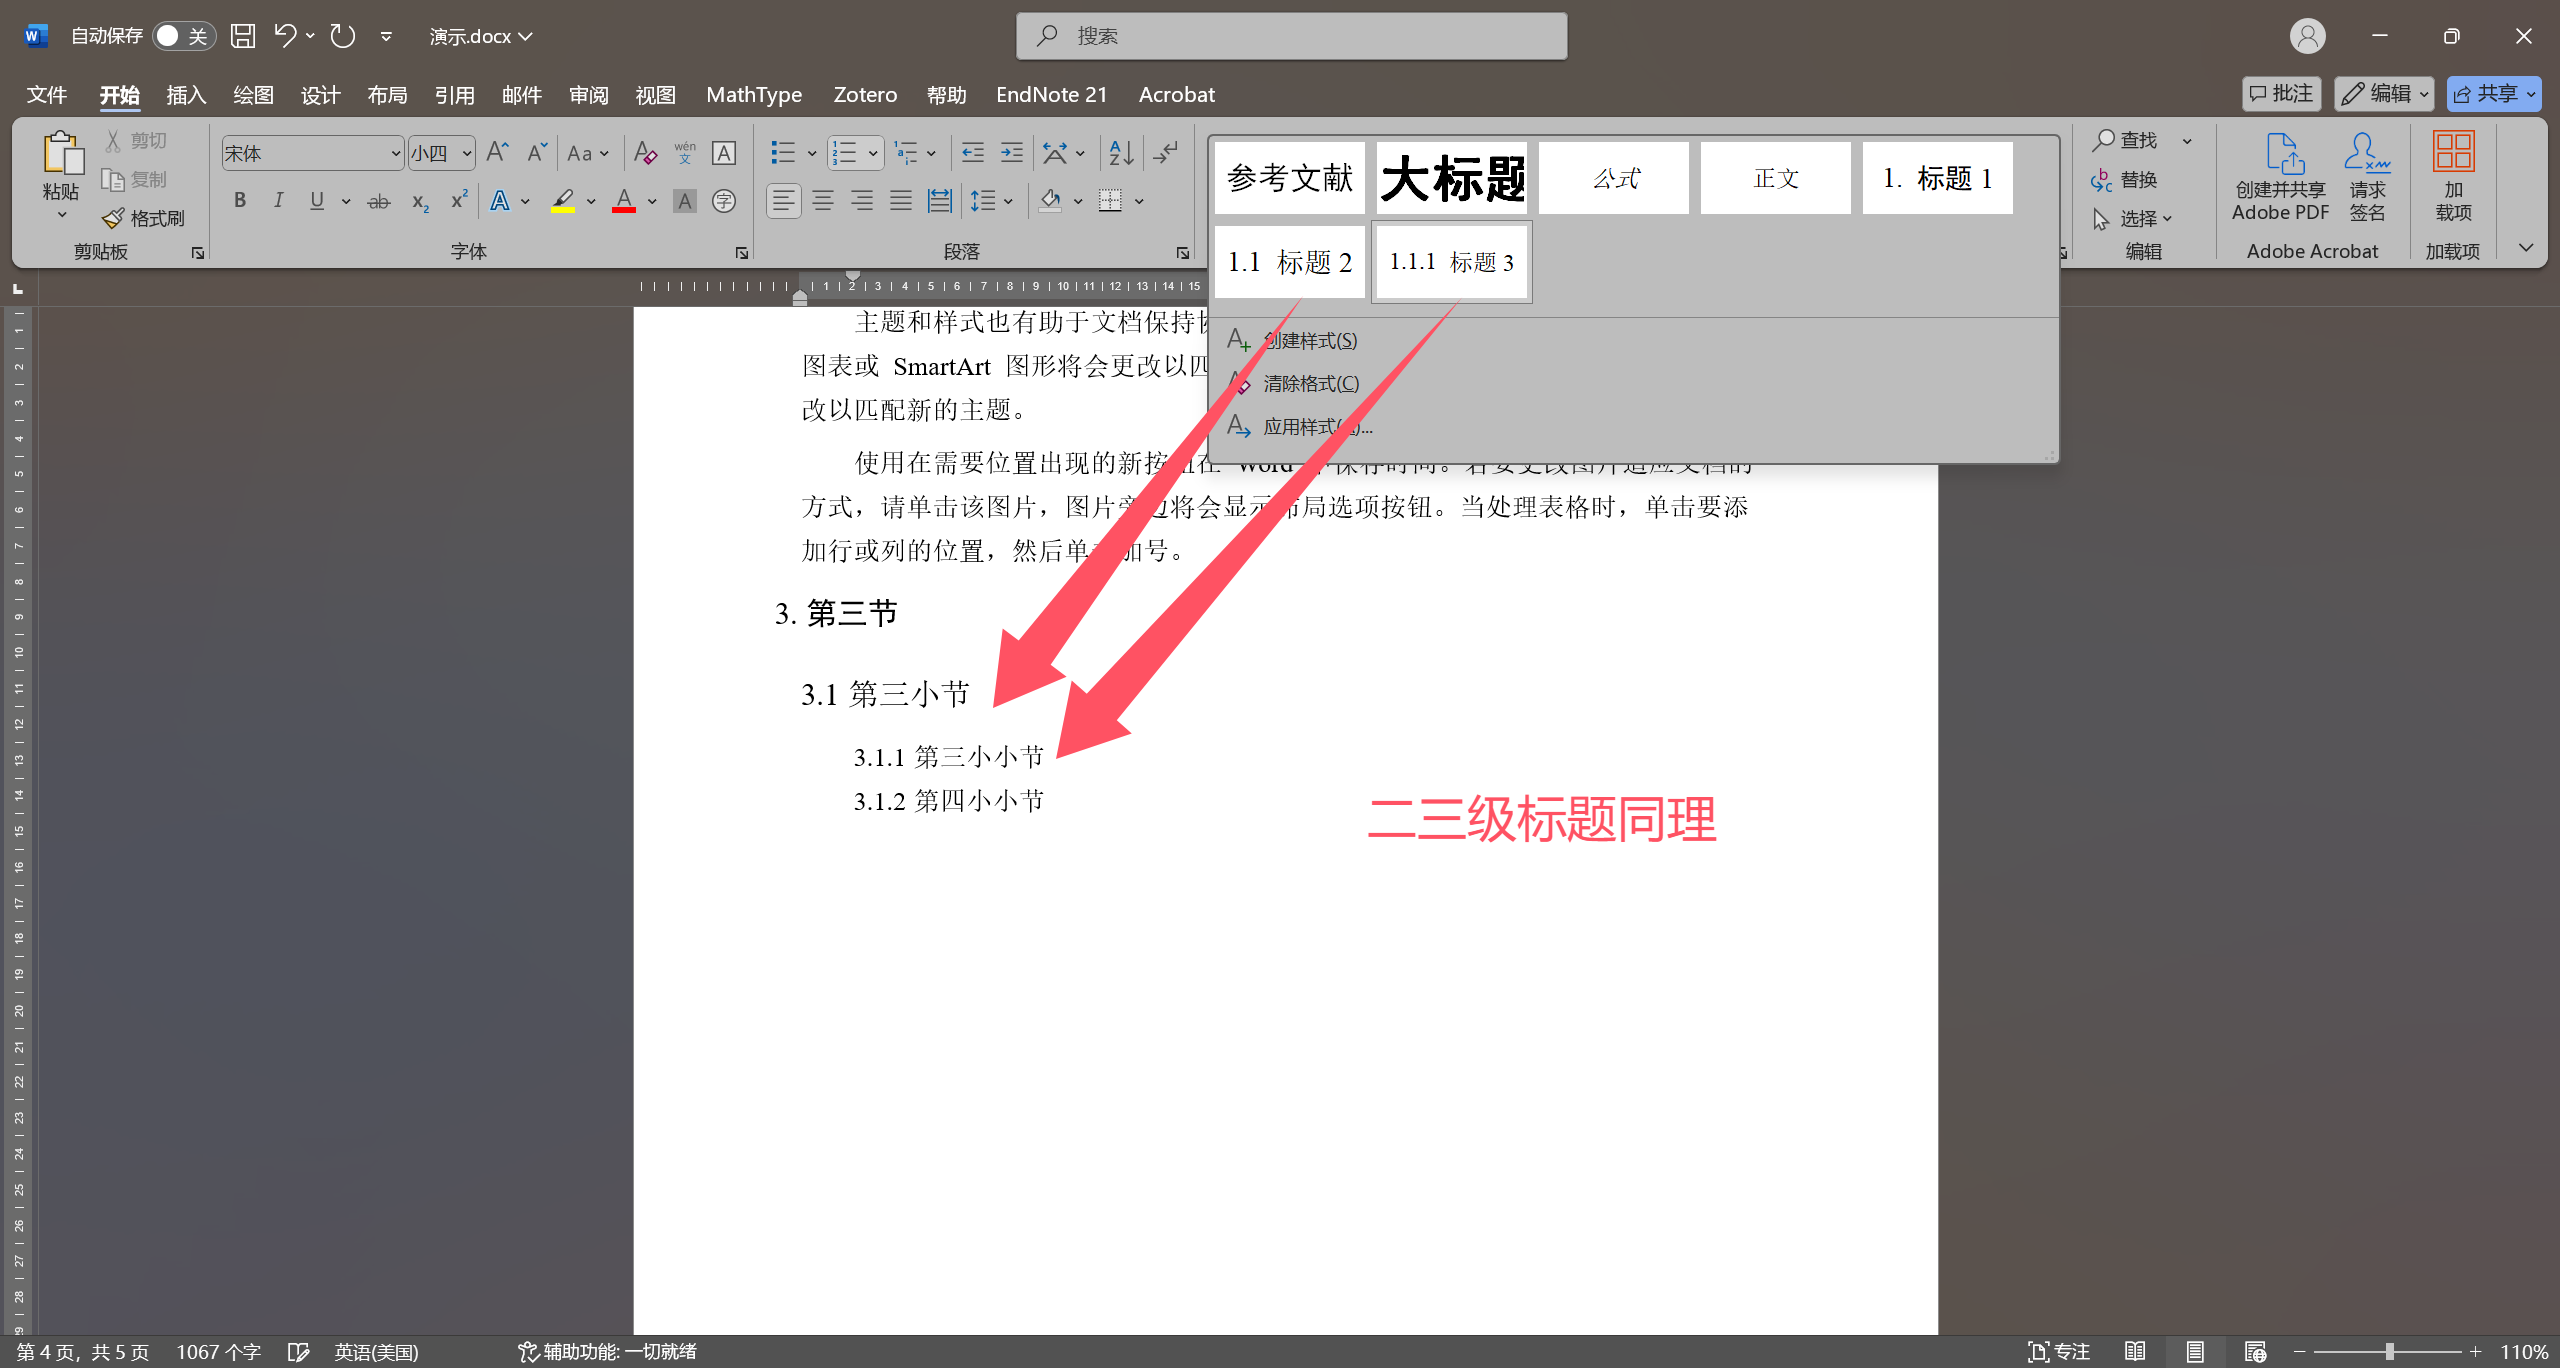
\includegraphics[width=\textwidth]{模板标题2.png}
    \caption{模板标题}
    \label{Word 2}
\end{figure}

\newpage

\subsection{目录}

我这个模板已经添加了目录,但它是不会自动更新的,

在添加新章节后,可以到“引用”选项卡,点击“更新目录”,
选择“更新整个目录”,即可更新目录:
\begin{figure}[!h]
    \centering
    \captionsetup{font={small, bf}, margin=60pt}
    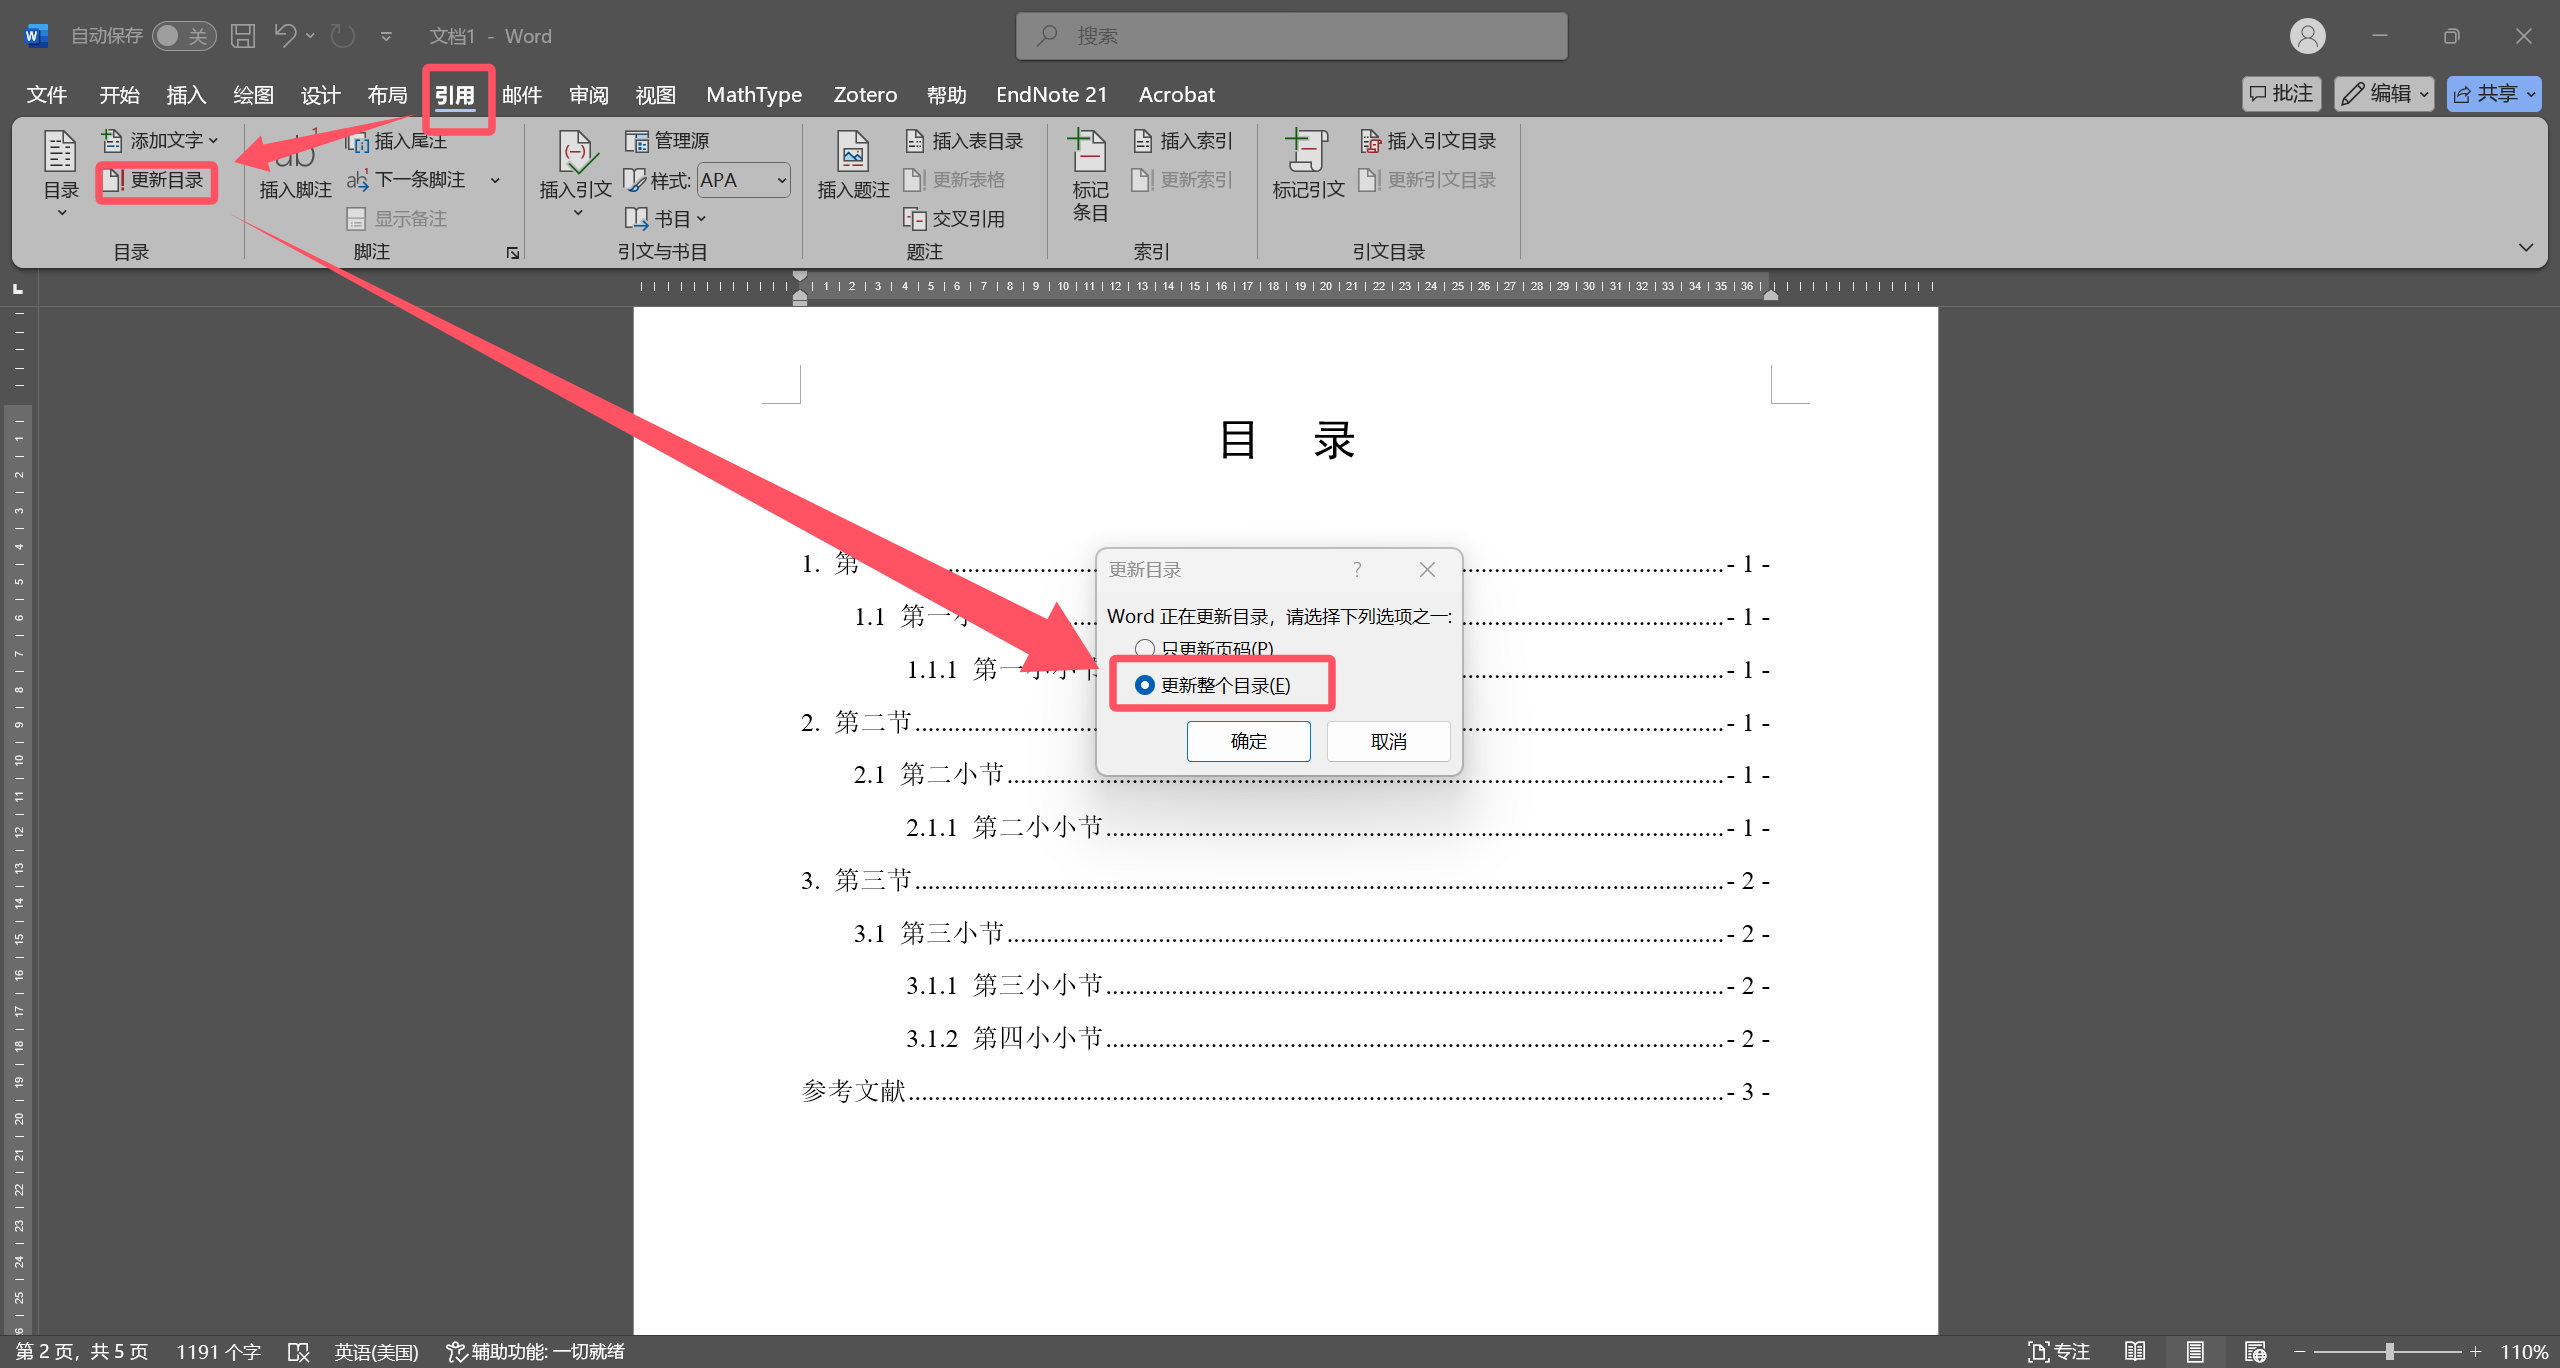
\includegraphics[width=\textwidth]{更新目录.png}
    \caption{更新目录}
    \label{Word 3}
\end{figure}

\subsection{在WPS中使用}
\subsubsection{WPS专业版下载}
我下载了多种WPS版本测试,发现专业版能够较好地兼容Zotero和公式,其它版本的WPS若没有启用宏,则无法使用Zotero。
学校购买了WPS专业版正版,可以在\textbf{\textcolor{blue}{\href{https://zbhrj1.jlu.edu.cn/download/wpsp.html}{吉大正版网站}}}直接下载使用。
在网站上有详细安装步骤,这里不再赘述。

注意安装时,可以更改安装路径,比如安装在“D:\backslash{}Kingsoft\backslash{}WPS Office”文件夹下。
另外,如果平时还是使用MS Office为主,可以在安装页面取消相关格式关联,或者在安装后也能在设置里更改。

\textbf{注意:在“WPS文字”中,大部分操作与Word相同,但有些操作会有所不同,在下面只介绍不同部分。}

\subsubsection{在WPS使用模板}
我提供的模板在WPS中也能使用,右击此模板文件,选择用“WPS文字”打开即可:
\begin{figure}[!h]
    \centering
    \captionsetup{font={small, bf}, margin=60pt}
    \begin{subfigure}[c]{0.9\textwidth}
    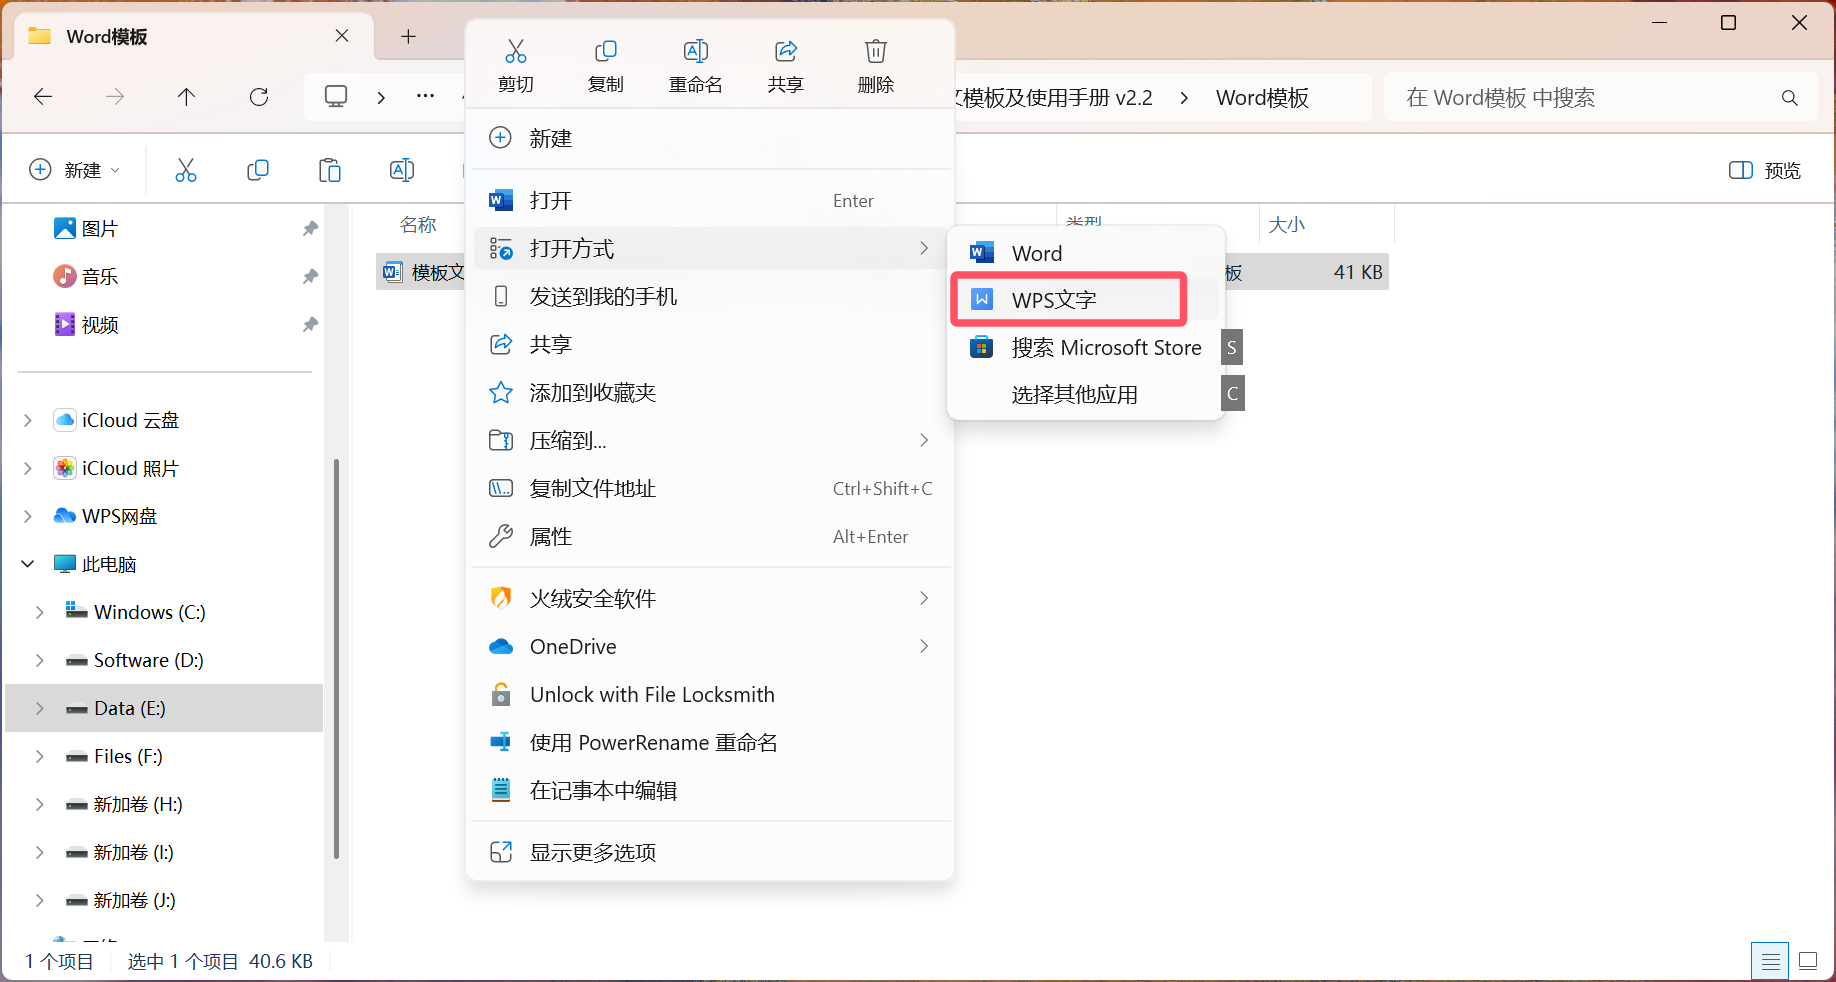
\includegraphics[width=\textwidth]{用WPS打开模板文件.png}
    \end{subfigure}    
    \caption{用WPS打开模板文件}
    \label{WPS 1}
\end{figure}

在WPS文字插入公式时,与Word不同的是,WPS默认所有字母和文字为正体,需要手动将一些字母改为斜体。可以选中后按快捷键Ctrl+I,快速切换正体与斜体。

另外,WPS内置了很多样式,下图里我把我模板里带的样式框起来了,与Word中一一对应,其中红色是使用得到的样式,操作方法与Word中相同:

\begin{figure}[!h]
    \centering
    \captionsetup{font={small, bf}, margin=60pt}
    \begin{subfigure}[c]{0.9\textwidth}
    
\includegraphics[width=\textwidth]{模板里的样式.png}
    \end{subfigure}    
    \caption{模板的样式}
    \label{WPS 2}
\end{figure}

\subsubsection{导出为PDF}

按下图所示,点击导出为PDF,检查输出路径和导出选项无误,即可导出:
\begin{figure}[h]
    \centering
    \captionsetup{font={small, bf}, margin=60pt}
    \begin{subfigure}[c]{0.6\textwidth}
      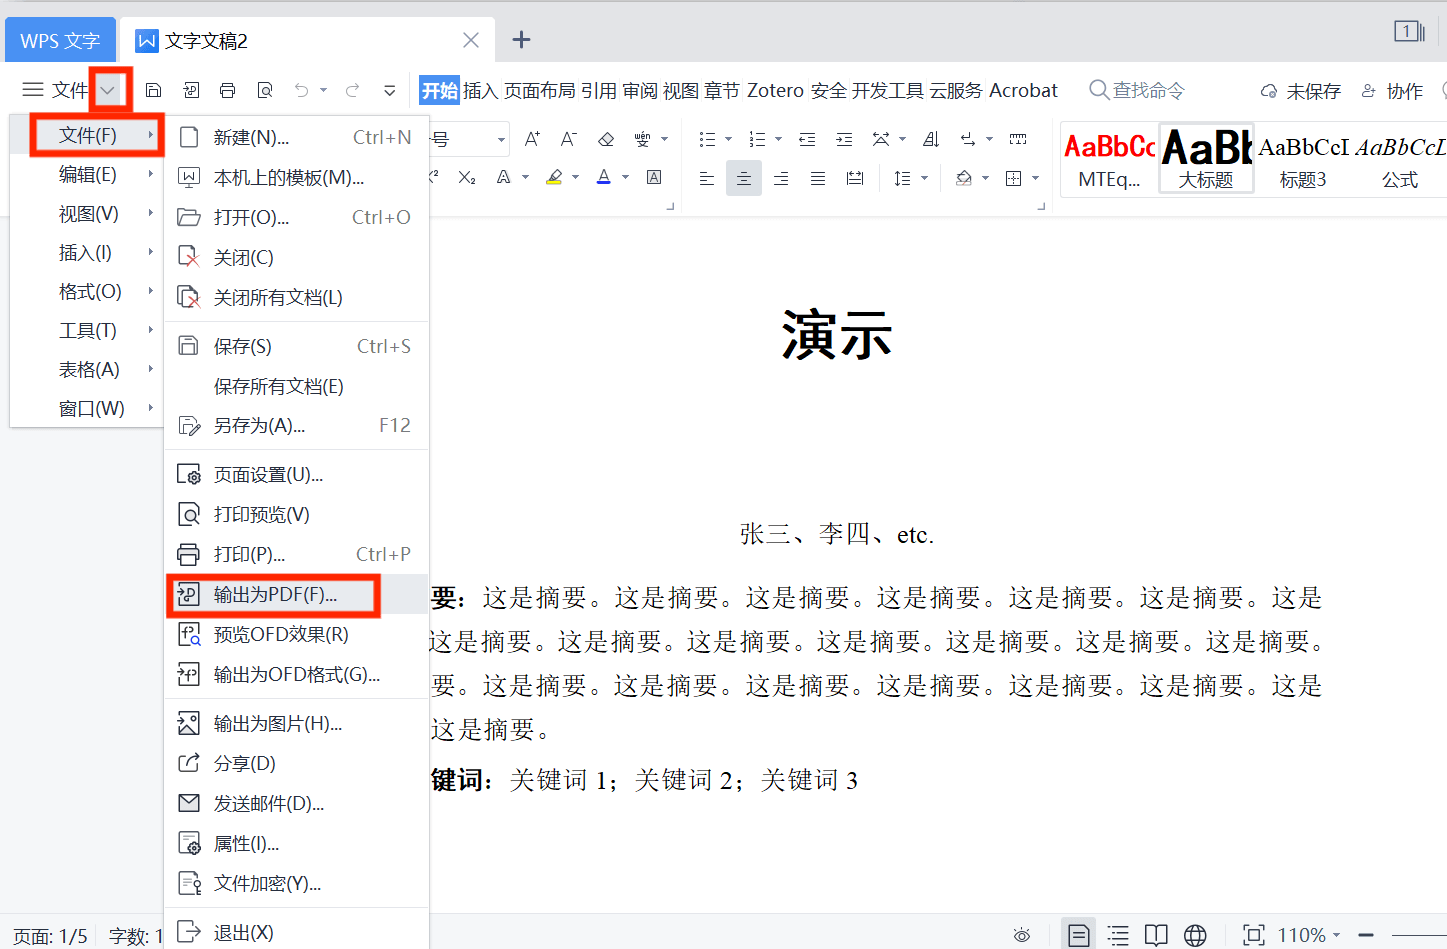
\includegraphics[width=\textwidth]{WPS导出为PDF.png}
    \end{subfigure}
    \hfill
    \begin{subfigure}[c]{0.35\textwidth}
      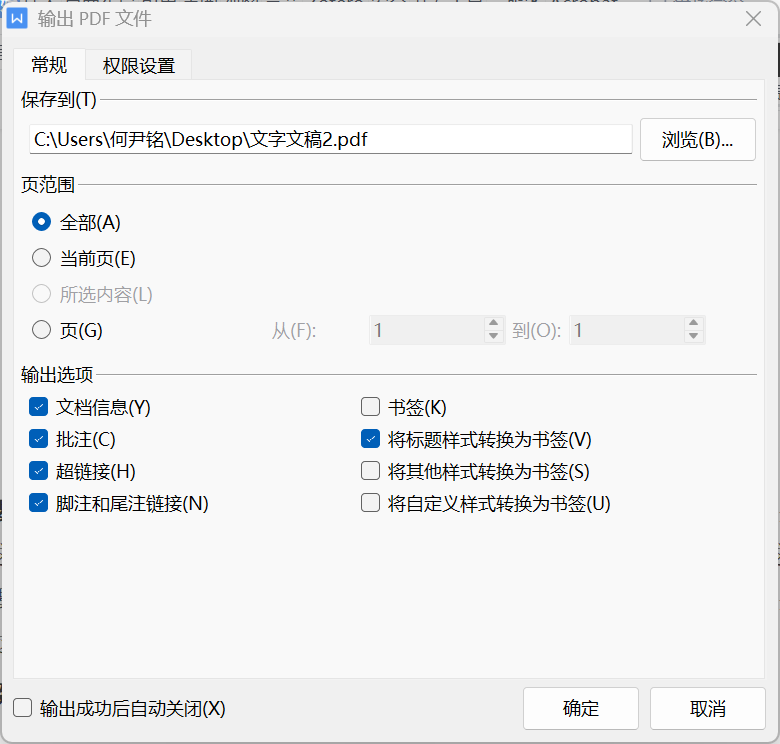
\includegraphics[width=\textwidth]{检查导出选项.png}
    \end{subfigure}
    \caption{WPS导出为PDF}
    \label{WPS 3}
\end{figure}

\subsection{碎碎念}
首行缩进2字符不要用空格!!!就算于吉红这么写我都照样骂(虽然她可能不在意就是了=\_=)。
本模板“正文”样式已经设置了首行缩进,也不需要手动设置。

这只是个很简陋的模板,但基本够用。
如果你有一定的Word基础,可以跟据自己喜好调整修改样式。

如果你对Word不熟悉,或者不想折腾,可以直接使用我这个模板。

希望我这个模板能带来一些帮助。
但事实上,用Word排版是远远不够的,
你在写论文时,如果遇到插入图片、图表,稍加调整,整篇文章可能就乱了。

不过,它所见即所得的编辑模式,对刚接触电脑的人很友好。
而且,如果你对Word十分熟悉,上面所提到的问题也都能解决,不过学习成本较高。

所以接下来,我将介绍更加专业的排版工具:\LaTeX。
\newpage
\section{\texorpdfstring{\LaTeX{} 入门}{LaTeX入门}} 
\subsection{\texorpdfstring{\LaTeX{} 简介及与Word对比}{Latex简介及与Word对比}}

\subsubsection{\texorpdfstring{\LaTeX{} 简介}{LaTeX简介}}

%\newcommand{\XeLaTeX}{X\kern-.15em\lower.5ex\hbox{\sffamily\small e}\kern-.05em\LaTeX}
\LaTeX{}是一个基于\TeX{}的排版系统,最初由Leslie Lamport于1984年开发。
它是一个开源的文档排版系统,广泛用于学术界和科研领域,尤其在数学、物理、计算机科学等领域中被广泛使用。
与传统的文字处理软件(如Word)相比,\LaTeX{}具有更强大的排版能力和灵活性,
特别是在处理复杂的数学公式、图表和参考文献时,有非常好的表现。

中文编写主要用\XeLaTeX{}编译器,
它是\LaTeX{}的一个扩展,支持Unicode字符集,可以更好地处理中文字符。
文档类型可选择“ctexart”,意为使用了“ctex”宏包的“article”文档类型。
我们不作过多介绍,够用即可。

\subsubsection{与Word对比}

\LaTeX{}与Word的所见即所得不同,写\LaTeX{}文件更像是在写代码,
实际上就是编写程序,告诉编译器如何排版,而在写作内容时,完全不需要考虑排版。

我看到过一个比喻:用Word就像是开小汽车,开得好不好、稳不稳,全凭驾驶员的技术;
而使用\LaTeX{}就像是开火车,一旦铺好了铁轨,车就会按照轨道稳定行驶,
但是,要铺好这个轨道需要较深厚的\LaTeX{}功底,我们一般都是使用别人铺好的轨道(即模板)。
我这里\textbf{只围绕我的模板进行介绍,讲解如何使用我的模板},更高级的技巧有兴趣可自行学习。

学习\LaTeX{}是个长期的过程,但一旦学习到一定程度,就会发现它相对于Word又快又好。
下面是一个\LaTeX{}和Word学习曲线图:
\begin{figure}[!h]
    \centering
    \captionsetup{font={small, bf}, margin=60pt}
    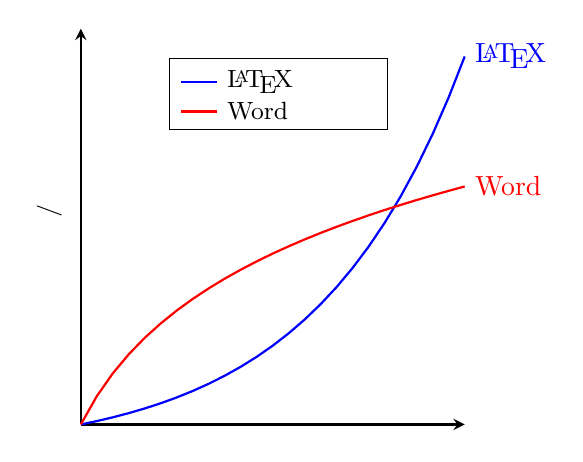
\begin{tikzpicture}[
        >=stealth,clip=true,scale=0.75
    ]
        \draw[->, thick] (0,0) -- (6.5,0) node[right] {\small 学习成本};
        \draw[->, thick] (0,0) -- (0,6.7) node[left, rotate=270, xshift=2.7cm, yshift=-0.4cm] {\small 熟练程度/效率};
    
        \draw[blue, thick, domain=0:6.5] 
            plot(\x, {(exp(0.4*\x) -1)*0.5}) node[right] {\LaTeX};
        \draw[red, thick, domain=0:6.5] 
            plot(\x, {(ln(\x +1))*2}) node[right] {Word};
    
        \draw[fill=white] (1.5,5) rectangle (5.2,6.2);
        \draw[blue,thick] (1.7,5.8) -- (2.3,5.8) node[right,black] {\small\LaTeX 曲线};
        \draw[red,thick] (1.7,5.3) -- (2.3,5.3) node[right,black] {\small Word曲线};
    
    \end{tikzpicture} 
    \caption{学习曲线对比图} 
\end{figure} 

\newpage

\subsection{下载安装及使用}
与其它语言相同,想要在自己电脑上编译、运行,就需要搭建运行环境。
我个人推荐使用VS Code代码编辑器,功能强大。

具体如何安装、配置,请参考\textbf{\textcolor{blue}{\href{https://zhuanlan.zhihu.com/p/38178015}{知乎文章(点击即可进入)}}}。

\textbf{注意,}一定要逐步按照文章内容,进行到最后一步。

另外VS Code界面支持中文,可以自己寻找教程修改。

正确安装并配置环境后,在VS Code左上角点击“文件”,选择“打开文件夹”,
这个文件夹就是工作文件夹了,所有编辑及编译的文件都在这个文件夹中。
你们可以选择我这个“演示”打开查看。

里面的文件就可以作为模板,把里面的文件拷贝到自己的工作文件夹,
在此基础上修改,就可直接应用模板的各种样式。

以我这个演示文件夹为例,其结构如下:
\begin{center}
\begin{minipage}{0.8\textwidth}
\dirtree{%
.1 演示/.
    .2 content/.
        .3 chapter1.tex.
        .3 \dots .
    .2 image/.
    .2 main.tex.
    .2 content.tex.
    .2 informatin.tex.
    .2 abstract.tex.
    .2 titlepage.tex.
    .2 apendendices.tex.
    .2 references.bib.
    .2 \dots .
}
\end{minipage}
\end{center}

理论上来说,\LaTeX{}文档一个文件足矣,我这样拆开是秉持着“样式与内容分离”的理念。

文档主要信息,如作者等在information.tex中编辑,摘要在abstract.tex中编辑。
附录我们用不到,我给它关掉了,需要用的话在主文件main.tex中打开(一般情况下不用打开main.tex),再编辑appendices.tex即可。

编写文档时,只需编辑content文件夹中的章节文件,然后再content.tex中添加所需文件即可。

参考文献以references.bib形式储存。图片储存在image文件夹中,其它文件就是辅助文件了。

main.pdf就是输出的文档。

\subsection{基础命令}
\subsubsection{章节与段落}

如果你只是编辑一些文字内容,可以直接在content文件夹中新建章节文件,
然后在content.tex中添加进去。

比如新建了一个chapter1.tex文件,在其中写入:
\begin{center}
\begin{minipage}{0.8\textwidth}
    \hspace{1em}
\begin{lstlisting}[language={[LaTeX]TeX}]
    \section{文献管理软件}
    \subsection{介绍}
    
    写论文最好有一个文献管理软件,方便管理参考文献。常用的有 EndNote、Mendeley、Zotero 等。
    我们学校已经购买了 Endnote 正版授权,可以到\textbf{\textcolor{blue}{\href{https://zbhrj1.jlu.edu.cn/download/EndNote21W.html}{吉大正版网站}}}下载使用。
    但是界面是全英文的,使用操作也不符合我的习惯,我这里只介绍我在用的Zotero,使用应该大同小异。
    
    
    
    \subsection{下载安装}
    
    Zotero基础功能免费,高级功能(如大容量云盘同步)是需要付费的,不过我们基本只用得到免费功能。
    软件可以在\textbf{\textcolor{blue}{\href{https://www.zotero.org/}{Zotero官方网站}}}直接下载使用。
\end{lstlisting}
\end{minipage}
\end{center}

\backslash section就是节标题,
同理\backslash subsection、\backslash subsubsection就是二三级节标题。
代码内换行编译出来是不换行的,换行在代码里体现是空一行,或者命令\backslash par。效果见本文档的效果见本文档开头(这就是本文档的代码)。
\\另外还有强制换行命令两个反斜杠\backslash\backslash ,但它只是换行,没有开启新的段落,这句话就是用了两个反斜杠换行的。

代码中的空格也不会参与编译,需要用到空格命令,这里介绍三种:

\begin{center}
\begin{minipage}{0.8\textwidth}
    \hspace{1em}
\begin{lstlisting}[language={[LaTeX]TeX}]
    a\qquad b % 两个字符空格

    a\quad b  % 一个字符空格 
    
    a\ b      % 小空格
\end{lstlisting}
\end{minipage}
\end{center}

效果如下:
\begin{center}
\begin{minipage}{0.8\textwidth}
a\qquad b 

a\quad b 

a\ b 
\end{minipage}
\end{center}

可以使用换页命令换页:
\begin{center}
\begin{minipage}{0.8\textwidth}
    \hspace{1em}
\begin{lstlisting}[language={[LaTeX]TeX}]
\newpage
\end{lstlisting}
\end{minipage}
\end{center}

\subsubsection{数学环境}

\LaTeX{}可以方便地输入美观的公式,下面介绍三种:

\begin{center}
\begin{minipage}{0.8\textwidth}
    \hspace{1em}
    \begin{lstlisting}[language={[LaTeX]TeX}]
        % 行内公式
        牛顿第二定律表述为:$F=ma$;
        % 单行不编号公式
        \[
            \int_{-1}^{1}x^2 \textrm{d}x=\frac{2}{3};
        \]
        % 单行编号公式
        \begin{equation}
            \int_{-1}^{1}x^2 \textrm{d}x=\frac{2}{3};
        \end{equation}
        % 多行编号公式
        \begin{align}
            \int_{-1}^{1}x^2 \textrm{d}x&=\left[\frac{1}{3}x^3\right]_{-1}^1\\
            &=\frac{2}{3}.
        \end{align}
\end{lstlisting}
\end{minipage}
\end{center}

效果如下:

牛顿第二定律表述为:$F=ma$;

\[
    \int_{-1}^{1}x^2 \textrm{d}x=\frac{2}{3};
\]

\begin{equation}
    \int_{-1}^{1}x^2 \textrm{d}x=\frac{2}{3};
\end{equation}

\begin{align}
    \int_{-1}^{1}x^2 \textrm{d}x&=\left[\frac{1}{3}x^3\right]_{-1}^1\\
    &=\frac{2}{3}.
\end{align}

如果要用无编号的equation或align,可替换成equation*或align*;
如果想要多行公式共用一个编号,可在equation中嵌套aligned。

\begin{center}
\begin{minipage}{0.8\textwidth}
    \hspace{1em}
\begin{lstlisting}[language={[LaTeX]TeX}]
        % 单行不编号公式
        \begin{equation}
            \int_{-1}^{1}x^2 \textrm{d}x=\frac{2}{3};
        \end{equation}
        % 多行单个编号公式
        \begin{equation}
            \begin{aligned}
                    \int_{-1}^{1}x^2 \textrm{d}x&=\left[\frac{1}{3}x^3\right]_{-1}^1\\
                    &=\frac{2}{3}
            \end{aligned}
        \end{equation}
\end{lstlisting}
\end{minipage}
\end{center}
    
效果如下:
\begin{equation*}
    \int_{-1}^{1}x^2 \textrm{d}x=\frac{2}{3};
\end{equation*}

\begin{equation}
\begin{aligned}
    \int_{-1}^{1}x^2 \textrm{d}x&=\left[\frac{1}{3}x^3\right]_{-1}^1\\
    &=\frac{2}{3}
\end{aligned}
\end{equation}

\subsection{稍稍进阶命令}

\begin{theorem}
    这是定理。
\end{theorem}

\begin{definition}
    这是定义。
\end{definition}

\begin{lemma}
    这是引理。
\end{lemma}

\begin{corollary}
    这是推论。    
\end{corollary}

\begin{example}
    这是例子。
\end{example}

\begin{proposition}
    这是命题。
\end{proposition}

实现代码如下:
\begin{center}
\begin{minipage}{0.8\textwidth}
    \hspace{1em}
\begin{lstlisting}[language={[LaTeX]TeX}]
    \begin{theorem}
        这是定理。
    \end{theorem}
    
    \begin{definition}
        这是定义。
    \end{definition}
    
    \begin{lemma}
        这是引理。
    \end{lemma}
    
    \begin{corollary}
        这是推论。    
    \end{corollary}
    
    \begin{example}
        这是例子。
    \end{example}
    
    \begin{proposition}
        这是命题。
    \end{proposition}
\end{lstlisting}
\end{minipage}
\end{center}

插入图片使用如下命令,效果见本文档\hyperref[Zotero 1]{开头}:
\begin{center}
\begin{minipage}{0.8\textwidth}
    \hspace{1em}
\begin{lstlisting}[language={[LaTeX]TeX}]
    \begin{figure}[htbp]
        \centering
        \captionsetup{font={small, bf}, margin=60pt}
        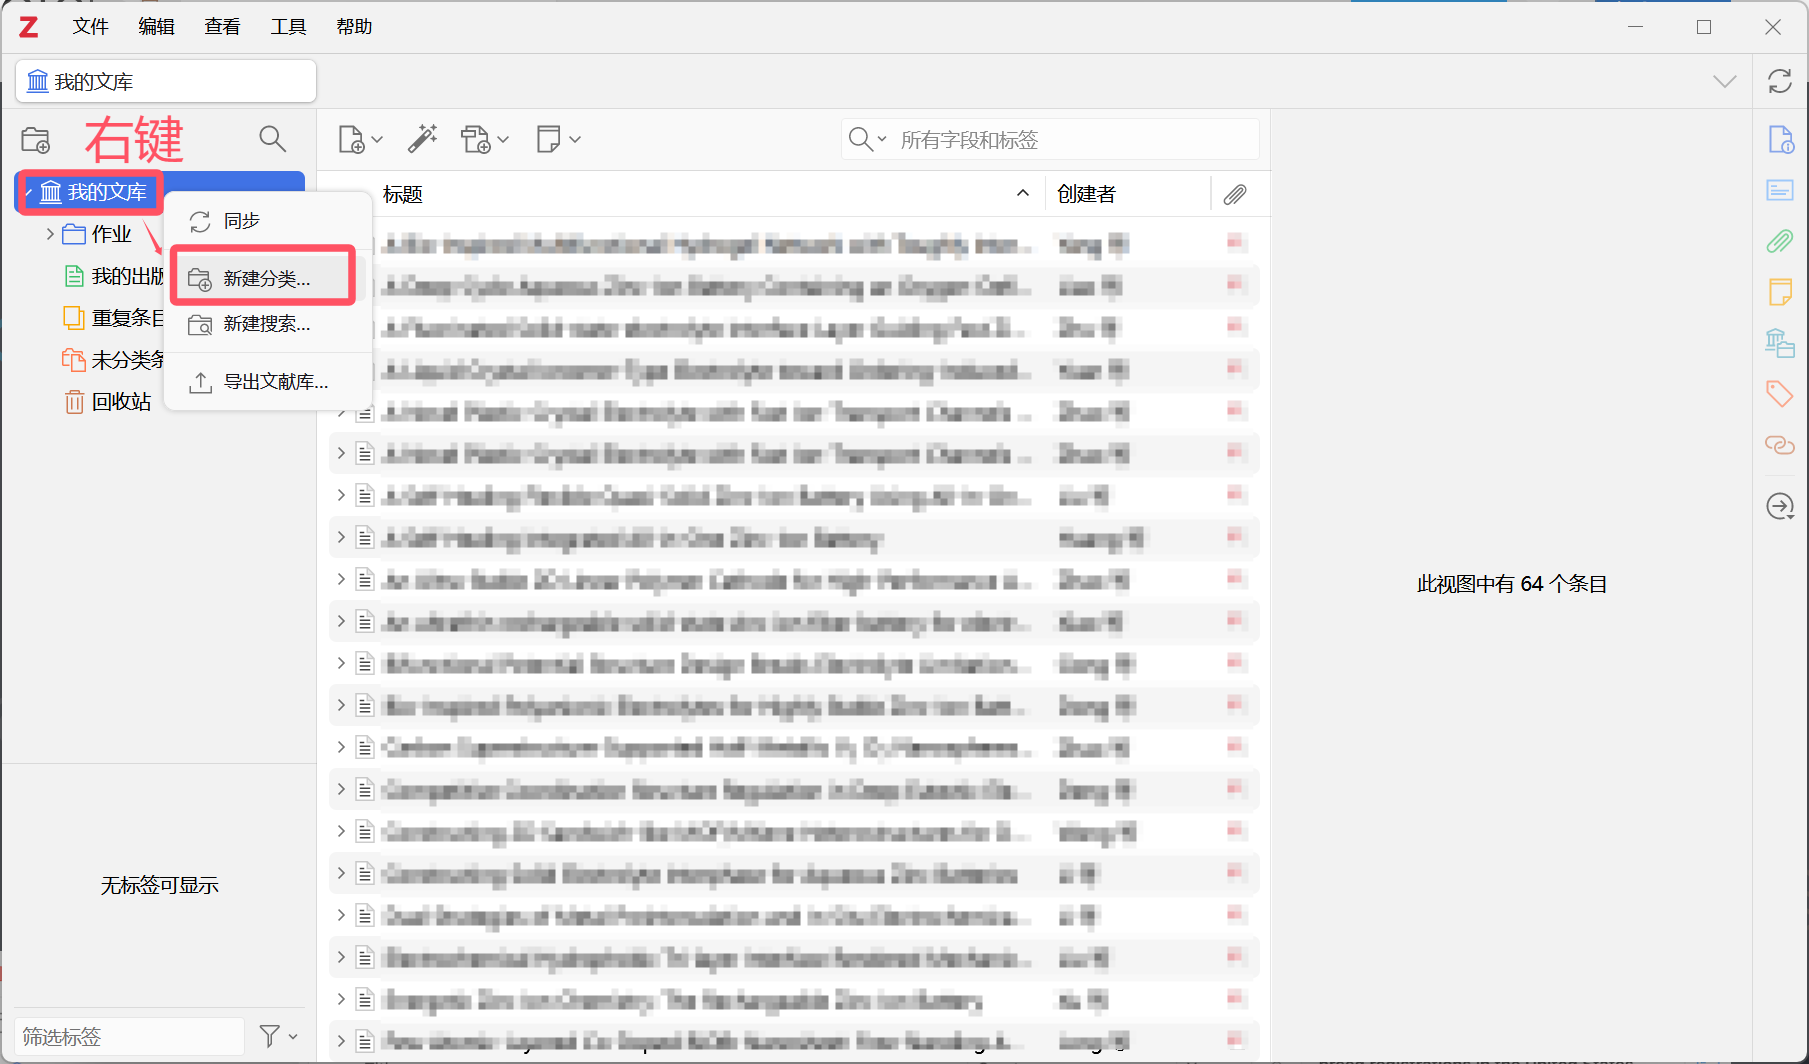
\includegraphics[width=0.8\textwidth]{Zotero打开.png}
        \caption{Zotero}
        \label{Zotero 1}
    \end{figure}
\end{lstlisting}
\end{minipage}
\end{center}

\newpage

\subsection{高阶命令}

\LaTeX{}可以实现很多你甚至想不到的功能。
随着学习的深入,你会认识到这是一个十分强大的工具。

高阶命令就不做介绍了,比如绘制表格、画图等等,有兴趣自行学习。

举个例子,\LaTeX{}中支持用TikZ绘图,精准但很麻烦。
在此不做介绍,只给出本文中例子,即学习曲线对比图:
\begin{center}
\begin{minipage}{0.8\textwidth}
    \hspace{1em}
\begin{lstlisting}[language={[LaTeX]TeX}]
    \begin{figure}[!h]
        \centering
        \captionsetup{font={small, bf}, margin=60pt}
        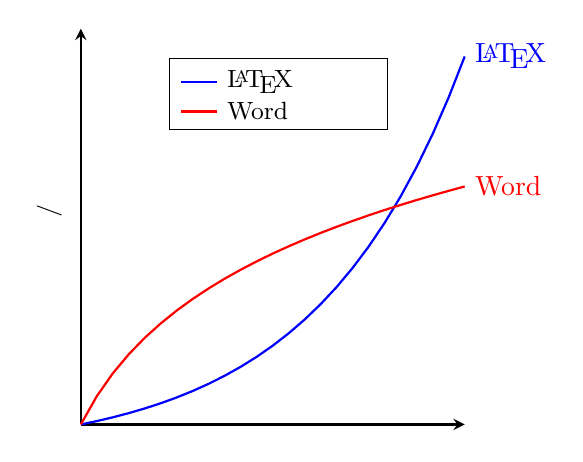
\begin{tikzpicture}[
            >=stealth,clip=true,scale=0.75
        ]
            \draw[->, thick] (0,0) -- (6.5,0) node[right] {\small 学习成本};
            \draw[->, thick] (0,0) -- (0,6.7) node[left, rotate=270, xshift=2.7cm, yshift=-0.4cm] {\small 熟练程度/效率};
        
            \draw[blue, thick, domain=0:6.5] 
                plot(\x, {(exp(0.4*\x) -1)*0.5}) node[right] {\LaTeX};
            \draw[red, thick, domain=0:6.5] 
                plot(\x, {(ln(\x +1))*2}) node[right] {Word};
        
            \draw[fill=white] (1.5,5) rectangle (5.2,6.2);
            \draw[blue,thick] (1.7,5.8) -- (2.3,5.8) node[right,black] {\small\LaTeX 曲线};
            \draw[red,thick] (1.7,5.3) -- (2.3,5.3) node[right,black] {\small Word曲线};
        
        \end{tikzpicture} 
        \caption{学习曲线对比图} 
    \end{figure} 
\end{lstlisting}
\end{minipage}
\end{center}

\newpage

\subsection{导入参考文献}

\newcommand{\BibTeX}{\textsc{B\kern-0.1emi\kern-0.017emb}\kern-0.15em\TeX}
\LaTeX{}可以方便地用\BibTeX{}管理参考文献,同样以Zotero为例,右键导出,选择\BibTeX{}(不选导出笔记),
导出到工作文件夹(这里是“演示”)为references.bib:

\begin{figure}[h]
    \centering
    \captionsetup{font={small, bf}, margin=60pt}
    \begin{subfigure}[c]{0.24\textwidth}
      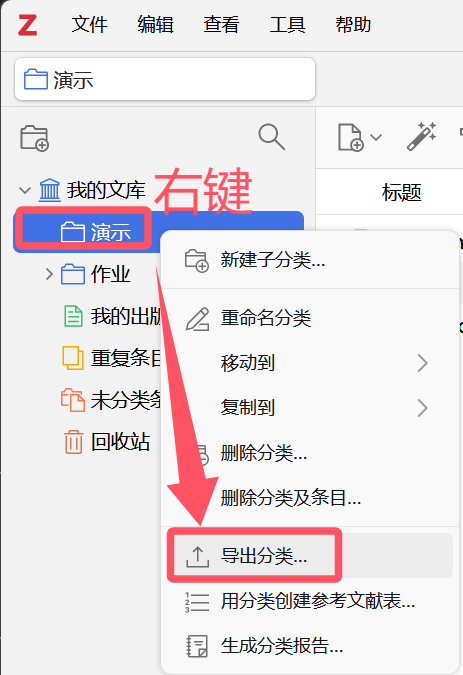
\includegraphics[width=\textwidth]{bib1.png}
      \label{bib 1-1}
    \end{subfigure}
    \hfill
    \begin{subfigure}[c]{0.20\textwidth}
      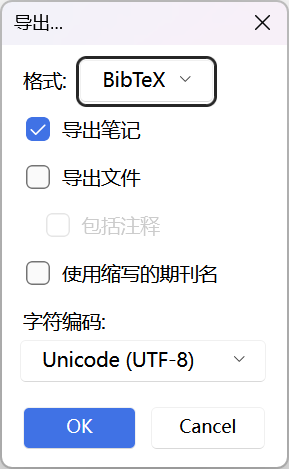
\includegraphics[width=\textwidth]{bib2.png}
      \label{bib 1-2}
    \end{subfigure}
    \hfill
    \begin{subfigure}[c]{0.47\textwidth}
      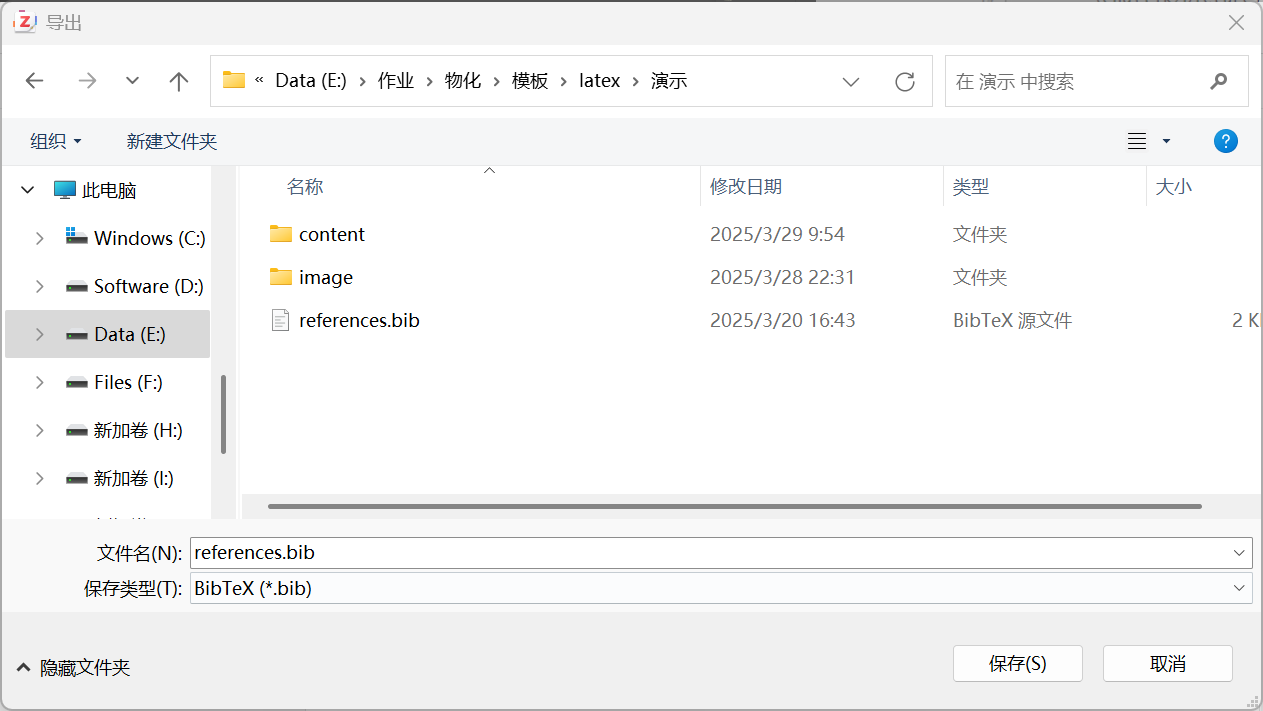
\includegraphics[width=\textwidth]{bib3.png}
      \label{bib 1-3}
    \end{subfigure}
    \caption{导出为references.bib}
    \label{bib 1}
\end{figure}

打开references.bib备用(可在VS Code里直接打开),
这次导入的第三个参考文献是从网页上直接导入的,里面有可以预先在Zotero文献信息中删除“其他”内容,
也可在references.bib文件手动删除“note=”这一行,以下即为\BibTeX{}文件(每个文献只展示前三行):

\begin{center}
\begin{minipage}{0.8\textwidth}
    \hspace{1em}
\begin{lstlisting}[language={[LaTeX]TeX}]
@article{zhao_novel_2023,
	title = {A {Novel} {Plastic}‐{Crystal} ...
	volume = {13},
    ...

@article{zhou_simultaneous_2024,
	title = {Simultaneous {Inhibition}...
	volume = {63},
    ...

@article{montes-tolentino_control_2025,
	title = {Control of {Interlocking} ...
	volume = {64},
    ...

\end{lstlisting}
\end{minipage}
\end{center}

\newcommand{\BibLaTeX}{\textsc{B\kern-0.1emi\kern-0.017emb}\kern-0.15em\LaTeX}
使用一些宏包能有其它的引用样式,也能调整是否显示链接或DOI等信息。这里不再赘述,可自行探索。

还可以使用更高级的\BibLaTeX{},可以通过参数直接调整想要显示的作者数量。这里不作演示,可自行学习。

引用时,bib文件中每条文献的第一行花括号右边就是标签,可以自行修改,但不建议(这里方便演示已分别改为a、b、c)。
按如下使用\backslash cite命令:
\begin{center}
\begin{minipage}{0.8\textwidth}
    \hspace{1em}
\begin{lstlisting}[language={[LaTeX]TeX}]
    示例文本:这里引用文献\cite{b},这里引用多个文献\cite{a, b, c}。
\end{lstlisting}
\end{minipage}
\end{center}
效果:

示例文本:这里引用文献\cite{b},这里引用多个文献\cite{a, b, c}。

同时,文档末尾会按照引用顺序生成引用文献列表,比如我这里的顺序是bac。
bib文献中有,但正文中未引用的文献也会排列在后面。

效果见本文档结尾。

还有更高级的交叉引用,如\backslash citet、\backslash citep、\backslash ref等等,
可以有多种引用,也可以引用文中的图片、表格等。这里不作介绍,可自行学习。

\subsection{编译}

编写好文档之后,如果你按照开头介绍的知乎文章正确配置的话,
就可以开始编译了,VS Code左边栏选择\TeX{},点击“构建\LaTeX{}项目”左边展开。

如果文章没有参考文献,点击\XeLaTeX{}开始编译,此时会报错,然后再点击编译一次,让章节信息进入目录即可。

如果文章有参考文献,点击\XeLaTeX{}->\BibTeX{}->\XeLaTeX{}*2,
一共会编译四次,第一次预编译,第二次导入参考文献,三四次则是执行两次正式编译,使目录也正常显示。
\section{其他高级排版软件}

你都用更高级的排版软件了,我这里也没必要废话了,

对吧(

(っ °\_°;)っ 


\newpage

% 参考文献
\nocite{*}
\bibliographystyle{unsrt}
\addcontentsline{toc}{section}{\refname}
\bibliography{references.bib}


\end{document}